\documentclass[11pt,letterpaper]{article}
\usepackage[utf8]{inputenc}
\usepackage[T1]{fontenc}
\DeclareUnicodeCharacter{00AC}{\ensuremath{\lnot}}
\DeclareUnicodeCharacter{00B0}{\ensuremath{^\circ}}
\usepackage[margin=2.2cm, top=2.4cm, bottom=2.4cm]{geometry}
\usepackage{graphicx}
\usepackage{booktabs}
\usepackage{array}
\usepackage{longtable}
\usepackage{float}
\usepackage{amsmath,amssymb}
\usepackage{xcolor}
\usepackage{fancyhdr}
\usepackage{hyperref}

\definecolor{uisgreen}{RGB}{27, 120, 55}
\definecolor{uisdark}{RGB}{0, 68, 27}
\definecolor{codebg}{RGB}{246, 248, 250}
\definecolor{linkblue}{RGB}{10, 88, 202}

\hypersetup{
    colorlinks=true,
    linkcolor=uisdark,
    urlcolor=linkblue,
    citecolor=uisdark,
    pdftitle={Informe Tarea 2 - Estadistica II - UIS},
    pdfauthor={Juan Jaimes, Marco Galvis, Maria Sarabia, Juan Prada}
}

\pagestyle{fancy}
\fancyhf{}
\fancyhead[L]{\footnotesize\textbf{UIS} — Estadística II (Tarea 2)}
\fancyhead[R]{\footnotesize J. Jaimes, M. Galvis, M. Sarabia, J. Prada}
\fancyfoot[C]{\small Página \thepage}
\renewcommand{\headrulewidth}{0.4pt}
\renewcommand{\footrulewidth}{0.4pt}

\renewcommand{\figurename}{Figura}
\renewcommand{\tablename}{Tabla}
\renewcommand{\contentsname}{Índice de Contenidos}

\setlength{\parskip}{0.45em}
\setlength{\parindent}{0pt}

\begin{document}

% -------------------- PORTADA --------------------
\begin{titlepage}
    \centering
    \vspace*{0.1cm}
    
\includegraphics[width=0.38\textwidth]{uis.png}\\[0.45cm]
    
    {\Large\textbf{UNIVERSIDAD INDUSTRIAL DE SANTANDER}}\\[0.12cm]
    {\large\textbf{FACULTAD DE CIENCIAS — ESCUELA DE MATEMÁTICAS}}\\[0.1cm]
    {\normalsize\textbf{BUCARAMANGA, SANTANDER}}\\[0.55cm]
    
    \rule{\textwidth}{1.4pt}\\[0.3cm]
    {\Large\textbf{TAREA 2: MODELOS DE REGRESIÓN LINEAL MÚLTIPLE Y REDES NEURONALES DE PERCEPTRÓN MULTICAPA EN PYTHON APLICADOS AL ANÁLISIS SOCIOECONÓMICO DEL EXAMEN ICFES SABER 11°}}\\[0.2cm]
    \rule{\textwidth}{1.4pt}\\[0.55cm]
    
    {\large\textbf{Asignatura:}} {\large Estadística II}\\[0.25cm]
    {\large\textbf{Profesor:}} {\large Dr. Andrés Ríos-Gutiérrez}\\[0.5cm]
    
    {\large\textbf{Integrantes del Grupo:}}\\[0.15cm]
    \begin{tabular}{c}
        \textbf{Juan Jaimes} \\
        \textbf{Marco Galvis} \\
        \textbf{Maria Sarabia} \\
        \textbf{Juan Prada}
    \end{tabular}\\[0.55cm]
    
    \fcolorbox{uisgreen}{codebg}{%
        \parbox{0.92\textwidth}{%
            \centering
            \vspace{0.15cm}
            \textbf{\color{uisdark}ENLACE AL REPOSITORIO Y CUADERNO JUPYTER EN GITHUB}\\[0.12cm]
            \footnotesize El código fuente completo, la base de datos \texttt{SB11\_20231.TXT}, las gráficas de alta resolución y el cuaderno interactivo \texttt{Tarea\_2\_Estadistica\_II.ipynb} con las interpretaciones línea a línea se encuentran disponibles en:\\[0.12cm]
            \textbf{Repositorio GitHub:} \href{https://github.com/juanes2809/Tarea-2-Estadistica-II}{\texttt{https://github.com/juanes2809/Tarea-2-Estadistica-II}}\\[0.06cm]
            \textbf{Cuaderno Jupyter:} \href{https://github.com/juanes2809/Tarea-2-Estadistica-II/blob/main/Tarea_2_Estadistica_II.ipynb}{\texttt{https://github.com/juanes2809/Tarea-2-Estadistica-II/blob/main/Tarea\_2\_Estadistica\_II.ipynb}}
            \vspace{0.15cm}
        }%
    }
    
    \vfill
    {\normalsize Bucaramanga, Colombia — 2026}
\end{titlepage}

\tableofcontents
\newpage

% -------------------- SECCIÓN 1 --------------------
\section{Introducción y Contexto de la Base de Datos (\texttt{SB11\_20231.TXT})}

\subsection{Origen de los Datos y Diseño Muestral/Poblacional}
El presente informe desarrolla un estudio estadístico riguroso sobre los determinantes académicos del nivel socioeconómico estudiantil en Colombia a partir de la base de datos oficial \texttt{SB11\_20231.TXT}, suministrada por el \textbf{Instituto Colombiano para la Evaluación de la Educación (ICFES)} dentro del programa de datos abiertos y la serie \textit{Saber al Detalle}. El archivo reúne los registros censales de la aplicación del \textbf{Examen de Estado de la Educación Media Saber 11° correspondiente al primer semestre de 2023 (cohorte 2023-1, Calendario B)}.

A diferencia de la prueba de Calendario A (que se aplica en el segundo semestre a más de 500,000 estudiantes de colegios mayoritariamente oficiales), la cohorte \texttt{2023-1} evalúa a la población de colegios de \textbf{Calendario B} y validantes del primer semestre. En términos computacionales, el archivo \texttt{SB11\_20231.TXT} es un fichero de texto plano delimitado por el carácter especial de negación lógica (\texttt{¬}), conformado exactamente por \textbf{$N = 12,704$ registros (estudiantes)} y \textbf{$83$ variables} que abarcan tres dimensiones:
\begin{enumerate}
    \item \textbf{Dimensión Sociodemográfica y Económica Familiar:} Incluye estrato de la vivienda (\texttt{FAMI\_ESTRATOVIVIENDA}), nivel educativo de los padres, ocupación parental, tenencia de bienes y conectividad (internet, computador, automóvil, número de libros) y el \textbf{Índice de Nivel Socioeconómico Individual (\texttt{ESTU\_INSE\_INDIVIDUAL})}.
    \item \textbf{Dimensión Institucional y Geográfica:} Naturaleza del colegio (\texttt{COLE\_NATURALEZA}: Oficial vs. No Oficial), carácter bilingüe (\texttt{COLE\_BILINGUE}), área de ubicación (Urbano vs. Rural) y departamento de residencia (\texttt{ESTU\_DEPTO\_RESIDE}), donde destacan Valle del Cauca ($6,288$ evaluados, $49.5\%$), Bogotá D.C. ($2,852$, $22.5\%$), Antioquia ($632$), Atlántico ($602$), Cauca ($590$), Cundinamarca ($501$) y \textbf{Santander ($168$ evaluados)}.
    \item \textbf{Dimensión de Desempeño Cognitivo (Pruebas Saber 11°):} Puntajes continuos discretizados en escala de $0$ a $100$ puntos (sin decimales) para las cinco áreas evaluadas por el ICFES, además del puntaje global (\texttt{PUNT\_GLOBAL}, escala de $0$ a $500$).
\end{enumerate}

\subsection{Definición de la Variable Respuesta y las Variables Explicativas}
En el marco de los modelos de regresión formulados en esta tarea, se establecen las siguientes variables:
\begin{itemize}
    \item \textbf{Variable Respuesta ($Y$): \texttt{ESTU\_INSE\_INDIVIDUAL}.} Es un índice continuo construido por el ICFES mediante un modelo de \textbf{Teoría de Respuesta al Ítem (TRI) de Crédito Parcial Generalizado} sobre las variables de capital cultural y físico del hogar reportadas en el formulario de inscripción. A nivel nacional (Calendario A+B), el índice se escala con media cercana a $50$ y desviación estándar de $10$, clasificándose en cuatro niveles socioeconómicos (\texttt{ESTU\_NSE\_INDIVIDUAL}): \textbf{NSE 1} ($\text{INSE} \le 40.99$), \textbf{NSE 2} ($41.00 \le \text{INSE} \le 51.20$), \textbf{NSE 3} ($51.21 \le \text{INSE} \le 62.89$) y \textbf{NSE 4} ($\text{INSE} \ge 62.90$).
    \item \textbf{Variables Explicativas Candidatas ($X_1, X_2, X_3, X_4, X_5$):}
    \begin{enumerate}
        \item \texttt{PUNT\_LECTURA\_CRITICA} ($X_1$): Evalúa comprensión literal, inferencial y crítica de textos continuos y discontinuos.
        \item \texttt{PUNT\_MATEMATICAS} ($X_2$): Evalúa interpretación, formulación, ejecución y argumentación cuantitativa.
        \item \texttt{PUNT\_C\_NATURALES} ($X_3$): Evalúa uso comprensivo del conocimiento científico, explicación de fenómenos e indagación en física, química, biología y ciencia-tecnología-sociedad (CTS).
        \item \texttt{PUNT\_SOCIALES\_CIUDADANAS} ($X_4$): Evalúa pensamiento social, interpretación de perspectivas y pensamiento reflexivo y sistémico.
        \item \texttt{PUNT\_INGLES} ($X_5$): Evalúa competencia comunicativa en lengua inglesa alineada con el Marco Común Europeo de Referencia (MCER: niveles A-, A1, A2, B1 y B+).
    \end{enumerate}
\end{itemize}

\subsection{Interpretación Línea a Línea de la Carga de Datos en Python}
En el cuaderno de Jupyter se implementa la lectura de la base de datos explicando cada instrucción requerida:
\begin{verbatim}
from google.colab import files # Importa la utilidad de carga de archivos en Google Colab
uploaded = files.upload()      # Almacena en diccionario el flujo binario del archivo subido
import pandas as pd            # Librería estándar para manejo de DataFrames tabulares
import io                      # Módulo para gestionar flujos de bytes en memoria RAM
datos_icfes = pd.read_csv(io.BytesIO(uploaded['SB11_20231.TXT']),
                          delimiter='¬') # Parsea el archivo separando columnas por '¬'
\end{verbatim}
Adicionalmente, el cuaderno incorpora detección automática mediante \texttt{os.path.exists('SB11\_20231.TXT')} con \texttt{engine='python'} para garantizar que el código se ejecute sin errores tanto en Google Colaboratory como en entornos locales y servidores de GitHub.

% -------------------- SECCIÓN 2 --------------------
\section{Eliminación de Valores Faltantes (\texttt{icfes\_sin\_nan}) y Justificación Estadística}

\subsection{Explicación Algorítmica Línea a Línea}
Para depurar los registros incompletos antes del modelado estadístico, se ejecuta el filtrado booleano vectorial sobre el objeto \texttt{datos\_icfes}:
\begin{verbatim}
icfes_sin_nan = datos_icfes[(~datos_icfes['ESTU_INSE_INDIVIDUAL'].isna()) &
                            (~datos_icfes['PUNT_LECTURA_CRITICA'].isna()) &
                            (~datos_icfes['PUNT_MATEMATICAS'].isna()) &
                            (~datos_icfes['PUNT_C_NATURALES'].isna()) &
                            (~datos_icfes['PUNT_SOCIALES_CIUDADANAS'].isna()) &
                            (~datos_icfes['PUNT_INGLES'].isna())]
\end{verbatim}
\textbf{Interpretación técnica:} El método \texttt{.isna()} genera una serie booleana donde \texttt{True} identifica celdas con valor nulo (\texttt{NaN}). El operador unario \texttt{\~{}} aplica la negación lógica bit a bit, transformando en \texttt{True} únicamente los registros con dato válido. Finalmente, el operador \texttt{\&} intersecta las seis condiciones exigiendo completitud simultánea en la variable respuesta y en las cinco variables explicativas.

\begin{table}[H]
\centering
\caption{Diagnóstico de valores faltantes y estadísticas descriptivas en \texttt{icfes\_sin\_nan} ($n = 11,853$).}
\label{tab:descriptivas}
\small
\resizebox{\textwidth}{!}{%
\begin{tabular}{lrrrrrrrrrr}
\toprule
\textbf{Variable} & \textbf{NaN} & \textbf{\% NaN} & \textbf{Media} & \textbf{DE} & \textbf{Mín} & \textbf{$Q_1$ (25\%)} & \textbf{Mediana} & \textbf{$Q_3$ (75\%)} & \textbf{Máx} & \textbf{Asimetría} \\
\midrule
\texttt{ESTU\_INSE\_INDIVIDUAL} & 849 & 6.68\% & 63.01 & 7.43 & 24.90 & 59.05 & 64.26 & 68.18 & 83.52 & $-0.643$ \\
\texttt{PUNT\_LECTURA\_CRITICA} & 0 & 0.00\% & 64.62 & 9.23 & 0.00 & 59.00 & 65.00 & 71.00 & 100.00 & $-0.387$ \\
\texttt{PUNT\_MATEMATICAS} & 0 & 0.00\% & 64.23 & 11.84 & 0.00 & 57.00 & 65.00 & 72.00 & 100.00 & $-0.172$ \\
\texttt{PUNT\_C\_NATURALES} & 0 & 0.00\% & 61.20 & 10.22 & 0.00 & 55.00 & 62.00 & 68.00 & 100.00 & $-0.398$ \\
\texttt{PUNT\_SOCIALES\_CIUDADANAS} & 0 & 0.00\% & 61.02 & 11.06 & 0.00 & 54.00 & 62.00 & 69.00 & 100.00 & $-0.495$ \\
\texttt{PUNT\_INGLES} & 2 & 0.02\% & 73.11 & 13.93 & 0.00 & 64.00 & 76.00 & 83.00 & 100.00 & $-0.477$ \\
\bottomrule
\end{tabular}%
}
\end{table}

\subsection{Justificación Estadística y Contextual de la Limpieza de Datos}
Como se documenta en la Tabla \ref{tab:descriptivas} , de los $12,704$ registros iniciales:
\begin{enumerate}
    \item \textbf{Subconjunto completo (\texttt{icfes\_sin\_nan}):} Conserva exactamente \textbf{$11,853$ estudiantes ($93.30\%$)} que cuentan con la totalidad de la información requerida.
    \item \textbf{Subconjunto sin INSE (\texttt{icfes\_connan}):} Comprende exactamente \textbf{$849$ estudiantes ($6.68\%$)} que presentaron las cinco pruebas cognitivas pero carecen de puntaje en \texttt{ESTU\_INSE\_INDIVIDUAL}. De acuerdo con la literatura metodológica del ICFES (Guía de Interpretación y Uso de Resultados Saber 11°) y la teoría de datos faltantes de Little y Rubin (2019), el índice INSE no se calcula cuando el estudiante deja en blanco los ítems del cuestionario sociodemográfico durante el registro en el sistema PRISMA. Al comparar las medias académicas de \texttt{icfes\_connan} ($\bar{X}_{\text{Inglés}} = 69.69$, $\bar{X}_{\text{Matemáticas}} = 61.11$) frente a las de \texttt{icfes\_sin\_nan} ($\bar{X}_{\text{Inglés}} = 73.11$, $\bar{X}_{\text{Matemáticas}} = 64.23$), se comprueba que la ausencia de respuesta no es completamente aleatoria (MCAR), sino \textbf{MAR (\textit{Missing At Random})}: depende sistemáticamente de variables observadas (el rendimiento académico). Si estos $849$ registros simplemente se descartaran sin imputación, se introduciría un sesgo de truncamiento hacia arriba en la estimación socioeconómica de la cohorte.
    \item \textbf{Registros con ausencia en pruebas académicas ($2$ casos, $0.02\%$):} Corresponden a dos evaluados que cuentan con INSE pero tienen valor nulo en \texttt{PUNT\_INGLES} por inasistencia a la segunda sesión del examen (donde se aplica el cuadernillo de Inglés). Su exclusión en la fase de entrenamiento e imputación es estadísticamente necesaria porque una variable explicativa faltante impide evaluar la función de regresión $\hat{Y} = f(X_1, \dots, X_5)$.
    \item \textbf{Valores atípicos y no representativos:} En el análisis exploratorio por cuantiles se identifican valores extremos inferiores (incluyendo puntajes de $0$ en pruebas individuales de estudiantes que anularon o dejaron en blanco un bloque específico) y una marcada asimetría negativa en todas las distribuciones ($\text{Skewness}$ entre $-0.17$ y $-0.64$). La media del INSE ($63.01$) y la mediana ($64.26$) ubican a más del $55\%$ de los estudiantes de esta cohorte en el nivel socioeconómico más alto (\textbf{NSE 4}, $\ge 62.90$), reflejando fielmente la composición socioeconómica de los colegios privados de Calendario B en Colombia.
\end{enumerate}



% -------------------- SECCIÓN 3 --------------------
\section{Selección de Variables Explicativas a partir de los Diagramas de Dispersión}

El primer criterio de selección de variables explicativas consiste en inspeccionar visual y analíticamente los diagramas de dispersión bivariados entre la variable respuesta \texttt{ESTU\_INSE\_INDIVIDUAL} (eje $Y$) y cada una de las cinco pruebas académicas (eje $X$). En la Figura \ref{fig:fig2} se presentan las cinco nubes de puntos ($n=11,853$) junto con sus rectas de regresión lineal simple estimadas por Mínimos Cuadrados Ordinarios ($\hat{Y} = \hat{\beta}_0 + \hat{\beta}_1 X_j$).

\begin{figure}[H]
    \centering
    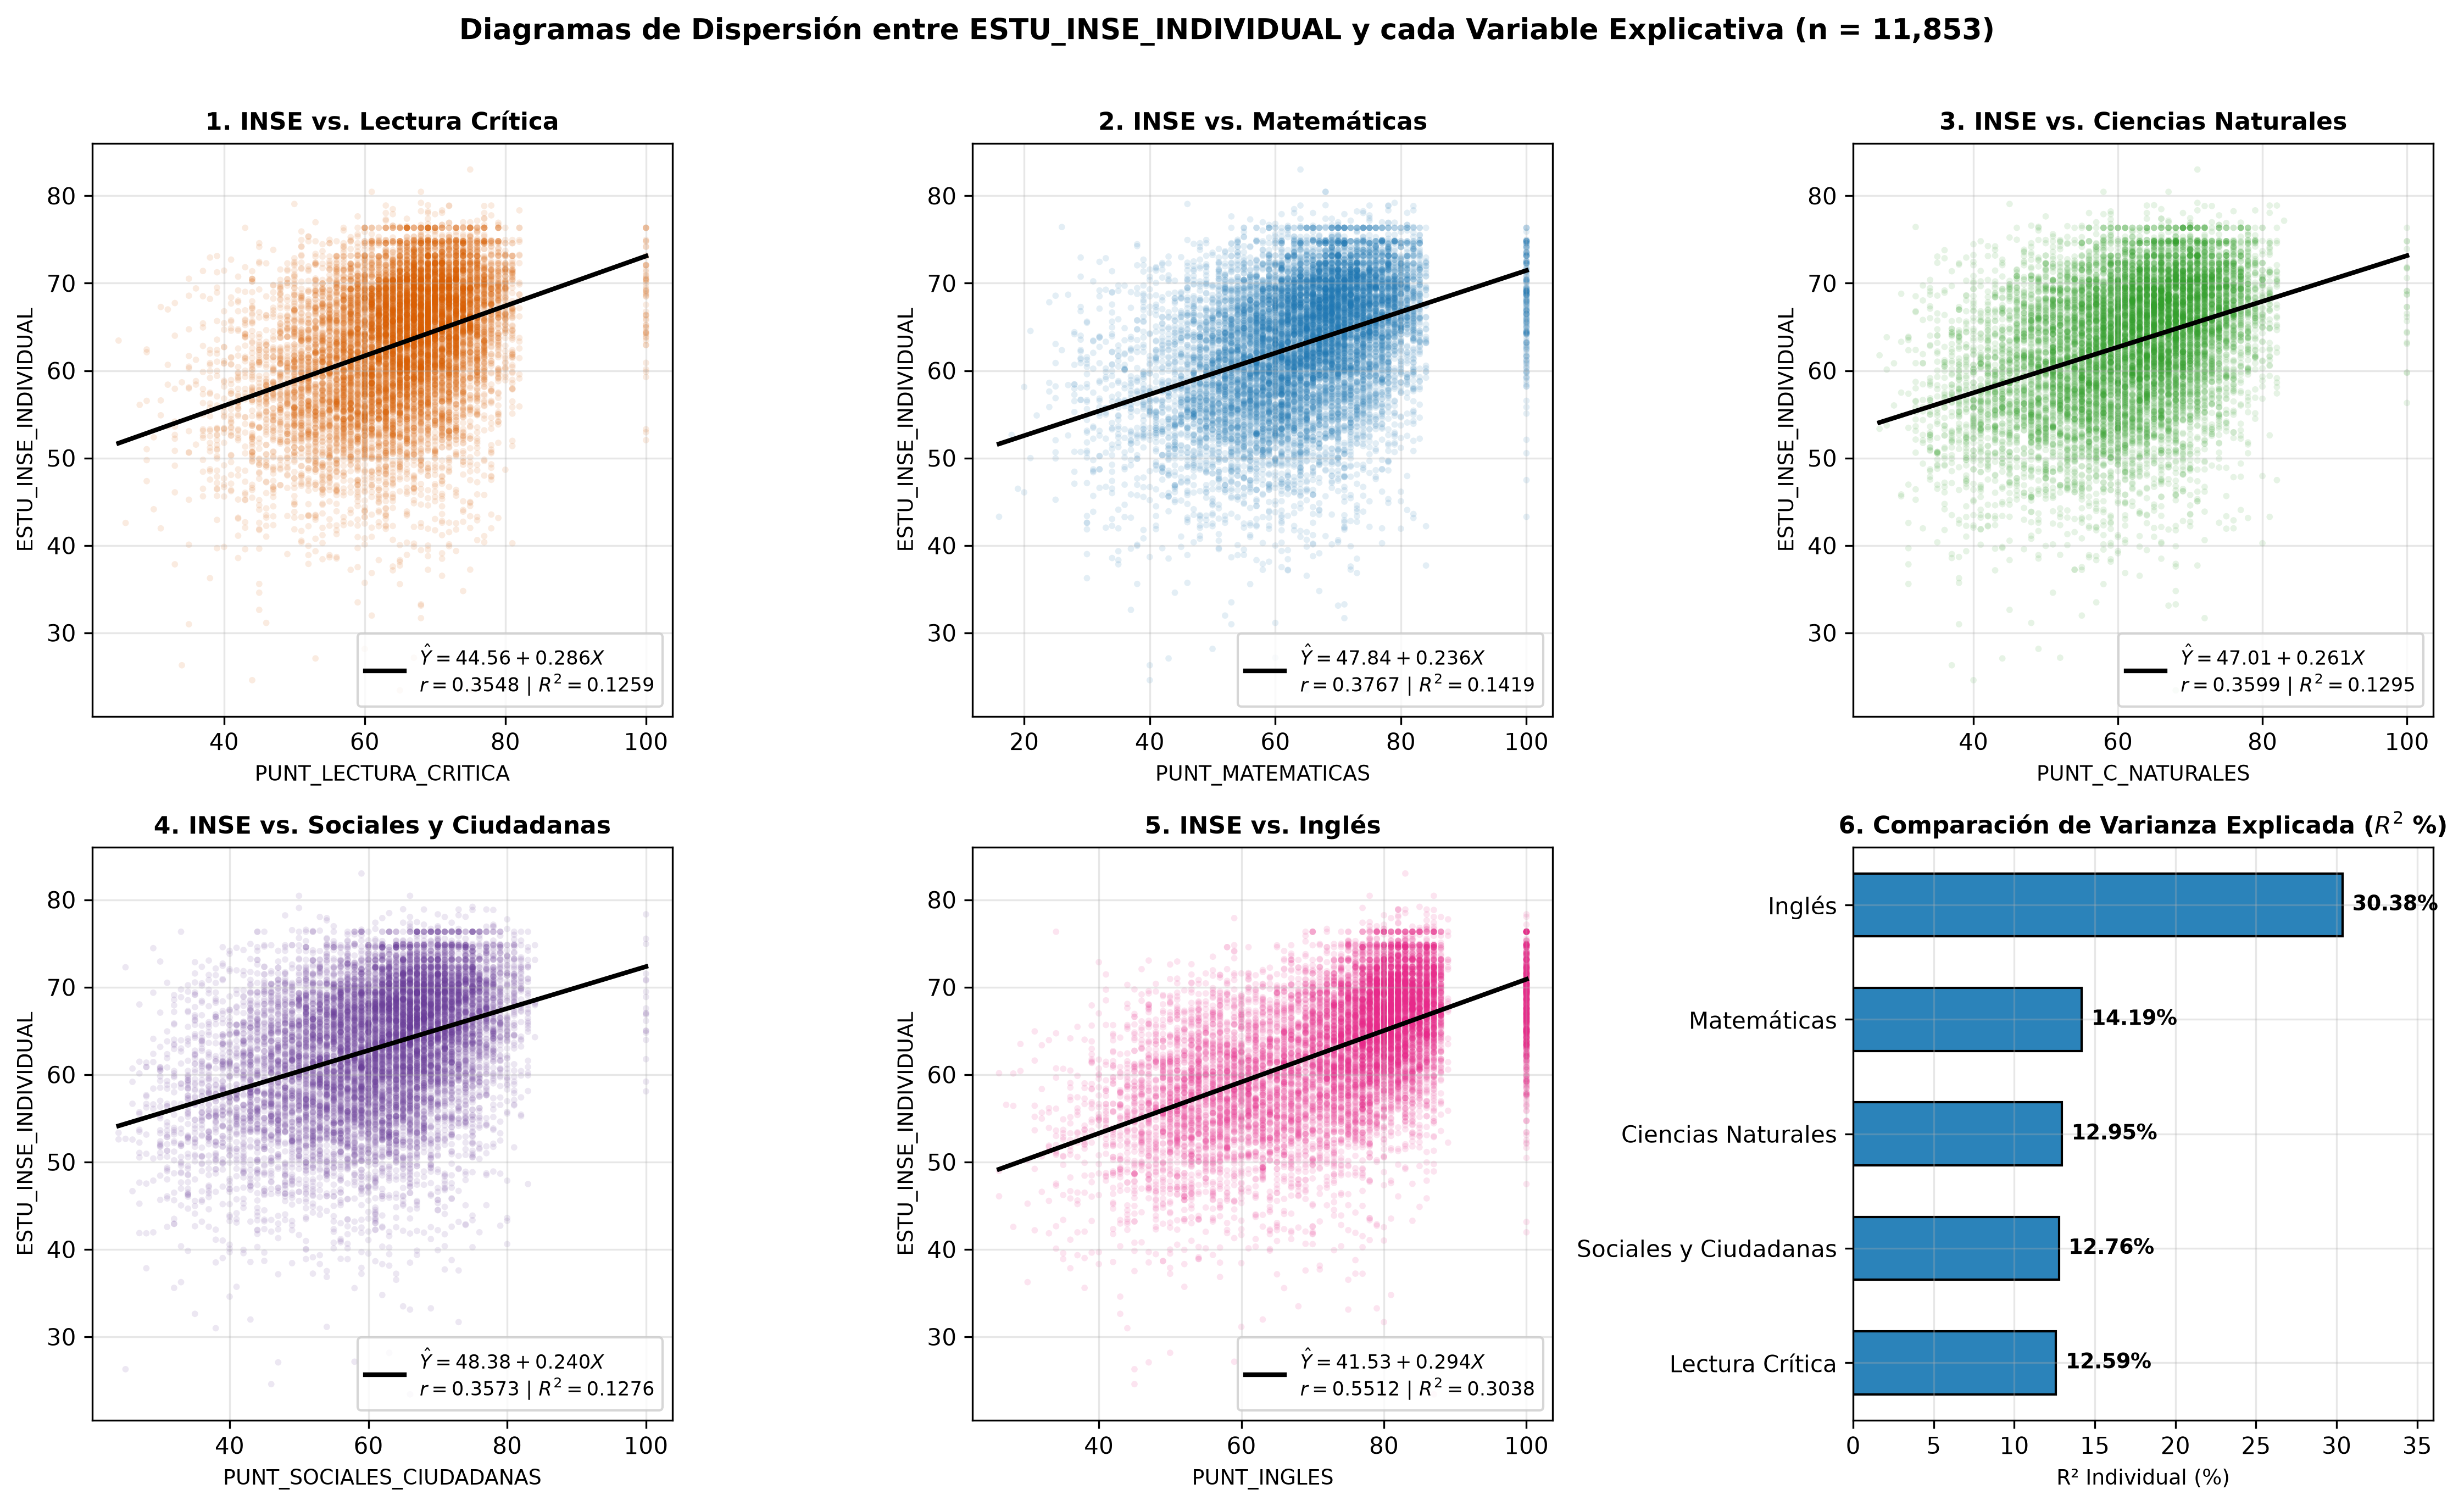
\includegraphics[width=0.99\textwidth]{figuras/fig2_diagramas_dispersion_2d.png}
    \caption{Diagramas de dispersión bivariados entre \texttt{ESTU\_INSE\_INDIVIDUAL} y cada una de las cinco variables explicativas candidatas, con rectas de regresión lineal simple y porcentaje de varianza explicada individual ($R^2$).}
    \label{fig:fig2}
\end{figure}

\textbf{Análisis estadístico de los diagramas de dispersión:}
\begin{enumerate}
    \item \textbf{\texttt{PUNT\_INGLES} (Panel 5):} Exhibe la relación lineal positiva más estrecha, empinada y definida de todo el conjunto ($\hat{\beta}_1 = 0.2937 \pm 0.0041$, $t = 71.91$, $p < 0.0001$). Por sí sola, la competencia en inglés explica el \textbf{$30.38\%$ de la variabilidad total del INSE ($R^2 = 0.3038$)}. Además, el diagrama evidencia una transición estructural: los estudiantes con puntajes entre $30$ y $55$ presentan alta dispersión socioeconómica ($\text{INSE} \in [35, 65]$), mientras que el segmento bilingüe ($\text{PUNT\_INGLES} \ge 80$) se concentra de forma compacta en la franja superior ($\text{INSE} \in [60, 80]$).
    \item \textbf{\texttt{PUNT\_MATEMATICAS} (Panel 2):} Constituye la segunda variable con mejor ajuste visual y analítico ($\hat{\beta}_1 = 0.2362 \pm 0.0053$, $t = 44.27$, $p < 0.0001$), explicando individualmente el \textbf{$14.19\%$ de la varianza ($R^2 = 0.1419$)}.
    \item \textbf{\texttt{PUNT\_C\_NATURALES} (Panel 3), \texttt{PUNT\_SOCIALES\_CIUDADANAS} (Panel 4) y \texttt{PUNT\_LECTURA\_CRITICA} (Panel 1):} Aunque las tres muestran pendientes positivas estadísticamente significativas ($\hat{\beta}_1 = 0.2615$, $0.2398$ y $0.2855$, respectivamente), sus nubes de puntos presentan una dispersión vertical considerablemente mayor alrededor de la recta de regresión, reflejada en coeficientes de determinación individuales más bajos y muy similares entre sí: \textbf{$12.95\%$}, \textbf{$12.76\%$} y \textbf{$12.59\%$}.
\end{enumerate}
Por consiguiente, el análisis gráfico bivariado selecciona en primer lugar a \textbf{\texttt{PUNT\_INGLES}} y en segundo lugar a \textbf{\texttt{PUNT\_MATEMATICAS}} como las variables explicativas dominantes.

% -------------------- SECCIÓN 4 --------------------
\section{Selección de Variables Explicativas a partir de los Coeficientes de Correlación de Pearson, de Kendall y de Spearman}

Para complementar la inspección visual con medidas formales de asociación invariantes a escala, se calcularon los tres coeficientes de correlación clásicos sobre \texttt{icfes\_sin\_nan} ($n = 11,853$):
\begin{itemize}
    \item \textbf{Correlación lineal de Pearson ($r$):} Evalúa la covarianza estandarizada $r_{XY} = \frac{\sum (x_i - \bar{x})(y_i - \bar{y})}{\sqrt{\sum (x_i - \bar{x})^2 \sum (y_i - \bar{y})^2}}$, óptima para relaciones lineales bajo normalidad bivariada.
    \item \textbf{Correlación por rangos Tau-b de Kendall ($\tau$):} Estadístico no paramétrico basado en la diferencia entre pares concordantes ($n_c$) y discordantes ($n_d$) ajustado por empates: $\tau = \frac{n_c - n_d}{\sqrt{(n_0 - n_1)(n_0 - n_2)}}$. Es sumamente robusto ante valores atípicos.
    \item \textbf{Correlación por rangos Rho de Spearman ($\rho$):} Evalúa la correlación de Pearson sobre los rangos asignados $R(X_i)$ y $R(Y_i)$, capturando cualquier relación monótona (lineal o no lineal).
\end{itemize}

\begin{table}[H]
\centering
\caption{Coeficientes de correlación de Pearson ($r$), Kendall ($\tau$) y Spearman ($\rho$) con \texttt{ESTU\_INSE\_INDIVIDUAL}.}
\label{tab:correlaciones}
\small
\resizebox{\textwidth}{!}{%
\begin{tabular}{clcccccc}
\toprule
\textbf{Orden} & \textbf{Variable Explicativa} & \textbf{Pearson ($r$)} & \textbf{Valor-$p$ ($r$)} & \textbf{Kendall ($\tau$)} & \textbf{Valor-$p$ ($\tau$)} & \textbf{Spearman ($\rho$)} & \textbf{Valor-$p$ ($\rho$)} \\
\midrule
1° & \texttt{PUNT\_INGLES} & \textbf{0.5512} & $< 10^{-300}$ & \textbf{0.3958} & $< 10^{-300}$ & \textbf{0.5657} & $< 10^{-300}$ \\
2° & \texttt{PUNT\_MATEMATICAS} & \textbf{0.3767} & $< 10^{-300}$ & \textbf{0.2711} & $< 10^{-300}$ & \textbf{0.3939} & $< 10^{-300}$ \\
3° & \texttt{PUNT\_C\_NATURALES} & 0.3599 & $< 10^{-300}$ & 0.2505 & $< 10^{-300}$ & 0.3647 & $< 10^{-300}$ \\
4° & \texttt{PUNT\_SOCIALES\_CIUDADANAS} & 0.3573 & $< 10^{-300}$ & 0.2488 & $< 10^{-300}$ & 0.3624 & $< 10^{-300}$ \\
5° & \texttt{PUNT\_LECTURA\_CRITICA} & 0.3548 & $< 10^{-300}$ & 0.2464 & $< 10^{-300}$ & 0.3576 & $< 10^{-300}$ \\
\bottomrule
\end{tabular}%
}
\end{table}



\textbf{Interpretación estadística de las matrices de correlación (Tabla \ref{tab:correlaciones}):}
\begin{enumerate}
    \item \textbf{Consistencia total del ranking:} Los tres criterios (paramétrico y no paramétricos) coinciden de forma unánime en el orden de las variables: \texttt{PUNT\_INGLES} lidera con amplia ventaja ($r = 0.5512$, $\rho = 0.5657$, $\tau = 0.3958$), superando en más de $17$ puntos porcentuales de correlación a la segunda variable, \texttt{PUNT\_MATEMATICAS} ($r = 0.3767$, $\rho = 0.3939$, $\tau = 0.2711$).
    \item \textbf{Superioridad sistemática de Spearman sobre Pearson ($\rho > r$):} En las cinco pruebas se verifica que $\rho > r$. Esto ocurre porque la relación entre el puntaje ICFES y el nivel socioeconómico presenta una leve concavidad en el extremo superior (los estudiantes de estrato 6 e $\text{INSE} > 75$ alcanzan el tope de $100$ puntos en inglés y matemáticas), por lo que la transformación por rangos de Spearman captura mejor la monotonía que el ajuste lineal estricto de Pearson. Asimismo, se verifica la relación teórica de Daniels-Kruskal ($\rho \approx \frac{3}{2}\tau$ para distribuciones cercanas a la normal bivariada).
    \item \textbf{Estructura de colinealidad inter-pruebas:} En la matriz de correlación de Pearson se observa que las cuatro pruebas en español (\texttt{PUNT\_LECTURA\_CRITICA}, \texttt{PUNT\_MATEMATICAS}, \texttt{PUNT\_C\_NATURALES} y \texttt{PUNT\_SOCIALES\_CIUDADANAS}) exhiben correlaciones mutuas muy elevadas: entre Ciencias Naturales y Matemáticas $r = 0.788$, entre Sociales y Lectura Crítica $r = 0.774$, y entre Ciencias Naturales y Sociales $r = 0.761$. En cambio, \texttt{PUNT\_INGLES} presenta correlaciones más moderadas con las demás pruebas ($r \in [0.626, 0.645]$). Esta estructura explica por qué Inglés aporta información socioeconómica diferenciada, mientras que las otras cuatro pruebas comparten un factor latente común de rendimiento escolar general.
\end{enumerate}

% -------------------- SECCIÓN 5 --------------------
\section{Selección de Variables Explicativas a partir del Coeficiente de Determinación ($R^2$) en Regresión Lineal Múltiple (Método ``Salvo Una'')}

Para determinar rigurosamente qué variables deben conservarse en un modelo multivariado, se estimó primero el \textbf{Modelo de Regresión Lineal Múltiple Completo} con las cinco variables explicativas:
\begin{equation}
\text{ESTU\_INSE\_INDIVIDUAL} = \beta_0 + \beta_1 X_{\text{LC}} + \beta_2 X_{\text{MAT}} + \beta_3 X_{\text{CN}} + \beta_4 X_{\text{SC}} + \beta_5 X_{\text{ING}} + \varepsilon
\end{equation}
obteniendo un coeficiente de determinación global de \textbf{$R^2_{\text{completo}} = 0.306011$} ($R^2_{\text{ajustado}} = 0.305718$, $F_{5, 11847} = 1044.8$, $p < 0.0001$). Acto seguido, se implementó el procedimiento de eliminación individual (\textit{leave-one-out covariate selection}): se ajustaron cinco modelos de regresión lineal múltiple incluyendo todas las variables explicativas \textbf{salvo una} ($R^2_{-j}$), midiendo la caída marginal $\Delta R^2_j = R^2_{\text{completo}} - R^2_{-j}$ y el estadístico $F$ parcial de cada predictor.

\begin{table}[H]
\centering
\caption{Selección de variables explicativas mediante el coeficiente de determinación ($R^2$) dejando fuera una variable a la vez ($\text{Modelo Completo: } R^2 = 0.306011, \; R^2_{\text{ajustado}} = 0.305718$).}
\label{tab:r2_salvo_una}
\small
\resizebox{\textwidth}{!}{%
\begin{tabular}{lccccccc}
\toprule
\textbf{Variable Omitida} & \textbf{$R^2$ sin la} & \textbf{$R^2$ Ajustado} & \textbf{Caída Marginal} & \textbf{Aporte al $R^2$} & \textbf{$F$ Parcial} & \textbf{Valor-$p$} & \textbf{\textquestiondown Es Explicativa en el} \\
\textbf{(``Salvo esta'')} & \textbf{Variable ($R^2_{-j}$)} & \textbf{sin la Variable} & \textbf{$\Delta R^2_j$} & \textbf{Total (\%)} & \textbf{($t_j^2$)} & \textbf{Marginal} & \textbf{Modelo Múltiple?} \\
\midrule
\texttt{PUNT\_INGLES} & \textbf{0.163901} & 0.163619 & \textbf{0.142109} & \textbf{46.44\%} & 2425.93 & $< 0.0001$ & \textbf{SÍ (1° Más Explicativa)} \\
\texttt{PUNT\_MATEMATICAS} & \textbf{0.304291} & 0.304056 & \textbf{0.001720} & \textbf{0.56\%} & 29.36 & $< 0.0001$ & \textbf{SÍ (2° Más Explicativa)} \\
\texttt{PUNT\_LECTURA\_CRITICA} & \textbf{0.305592} & 0.305358 & \textbf{0.000419} & \textbf{0.14\%} & 7.15 & $0.0075$ & \textbf{SÍ (3° Significativa)} \\
\texttt{PUNT\_C\_NATURALES} & 0.305966 & \textbf{0.305731} & 0.000045 & 0.01\% & 0.77 & $0.3806$ & NO (Redundante, $p > 0.05$) \\
\texttt{PUNT\_SOCIALES\_CIUDADANAS} & 0.305984 & \textbf{0.305750} & 0.000026 & 0.01\% & 0.45 & $0.5040$ & NO (Redundante, $p > 0.05$) \\
\bottomrule
\end{tabular}%
}
\end{table}



\textbf{Análisis profundo de los resultados de selección por $R^2$ (Tabla \ref{tab:r2_salvo_una}):}
\begin{enumerate}
    \item \textbf{Contraste crucial entre correlación bivariada y regresión múltiple:} Mientras que en los diagramas de dispersión y correlaciones simples las variables \texttt{PUNT\_C\_NATURALES} ($r=0.3599$) y \texttt{PUNT\_SOCIALES\_CIUDADANAS} ($r=0.3573$) parecían ocupar el tercer y cuarto lugar, en el modelo de regresión lineal múltiple \textbf{ambas pierden por completo su significancia estadística} ($p = 0.3806$ y $p = 0.5040$, con aportes marginales $\Delta R^2 < 0.00005$). De hecho, al eliminar cualquiera de las dos, el $R^2$ ajustado \textbf{aumenta} respecto al modelo completo (pasando de $0.305718$ a $0.305731$ y $0.305750$, y llegando a un máximo de \textbf{$0.305782$} cuando se eliminan ambas simultáneamente). Esto se explica por sus elevados Factores de Inflación de la Varianza ($\text{VIF}_{\text{CN}} = 3.90$ y $\text{VIF}_{\text{SC}} = 3.45$): toda su varianza compartida con el nivel socioeconómico ya es absorbida por Inglés, Matemáticas y Lectura Crítica.
    \item \textbf{Dominancia absoluta de \texttt{PUNT\_INGLES}:} Sin el puntaje de inglés, el $R^2$ del modelo con las otras cuatro pruebas cae de $0.306011$ a $0.163901$ ($\Delta R^2 = 0.142109$). Esto demuestra que casi la mitad ($46.44\%$) de la capacidad explicativa del modelo proviene exclusivamente de la información única que aporta \texttt{PUNT\_INGLES} ($\text{VIF}_{\text{ING}} = 1.98$, el más bajo de todos).
    \item \textbf{Las dos variables más explicativas:} De acuerdo con la caída en $R^2$, las dos variables más explicativas son inequívocamente \textbf{\texttt{PUNT\_INGLES}} ($\Delta R^2 = 0.142109$, $F = 2425.93$) y \textbf{\texttt{PUNT\_MATEMATICAS}} ($\Delta R^2 = 0.001720$, $F = 29.36$). Juntas alcanzan un $R^2 = 0.305405$ (el \textbf{$99.80\%$} de todo el poder explicativo del modelo de 5 variables).
    \item \textbf{Efecto supresor clásico de \texttt{PUNT\_LECTURA\_CRITICA}:} Resulta sumamente interesante desde la teoría econométrica que \texttt{PUNT\_LECTURA\_CRITICA} sea la tercera variable significativa ($p = 0.0075$, $\Delta R^2 = 0.000419$) con un coeficiente parcial negativo ($\hat{\beta}_{\text{LC}} = -0.0286$). En estadística multivariada (Conger, 1974), esto se denomina \textit{efecto supresor}: a igualdad de puntaje en Inglés y Matemáticas, un estudiante con puntaje sobresaliente en Lectura Crítica suele provenir de colegios públicos o de clase media con alto hábito lector pero menor capital económico relativo que aquellos cuyo puntaje alto se concentra exclusivamente en el bilingüismo.
\end{enumerate}

% -------------------- SECCIÓN 6 --------------------
\section{Diagrama con el Plano de Dispersión 3D (\texttt{ESTU\_INSE\_INDIVIDUAL} y las Dos Variables Más Explicativas)}

Seleccionadas \textbf{\texttt{PUNT\_INGLES}} ($X_1$) y \textbf{\texttt{PUNT\_MATEMATICAS}} ($X_2$) como las dos variables más explicativas, se estimó el modelo de regresión lineal múltiple tridimensional sobre la totalidad de \texttt{icfes\_sin\_nan} ($n = 11,853$):
\begin{equation}
\widehat{\text{ESTU\_INSE\_INDIVIDUAL}} = 40.7107 + 0.2764\,\text{PUNT\_INGLES} + 0.0325\,\text{PUNT\_MATEMATICAS}
\end{equation}
con errores estándar $\text{EE}(\hat{\beta}_0) = 0.347$, $\text{EE}(\hat{\beta}_1) = 0.0051$ ($t = 54.63, p < 0.0001$) y $\text{EE}(\hat{\beta}_2) = 0.0060$ ($t = 5.45, p < 0.0001$), alcanzando un coeficiente de determinación de \textbf{$R^2 = 0.305405$} ($F_{2, 11850} = 2605.0, p < 0.0001$).

\begin{figure}[H]
    \centering
    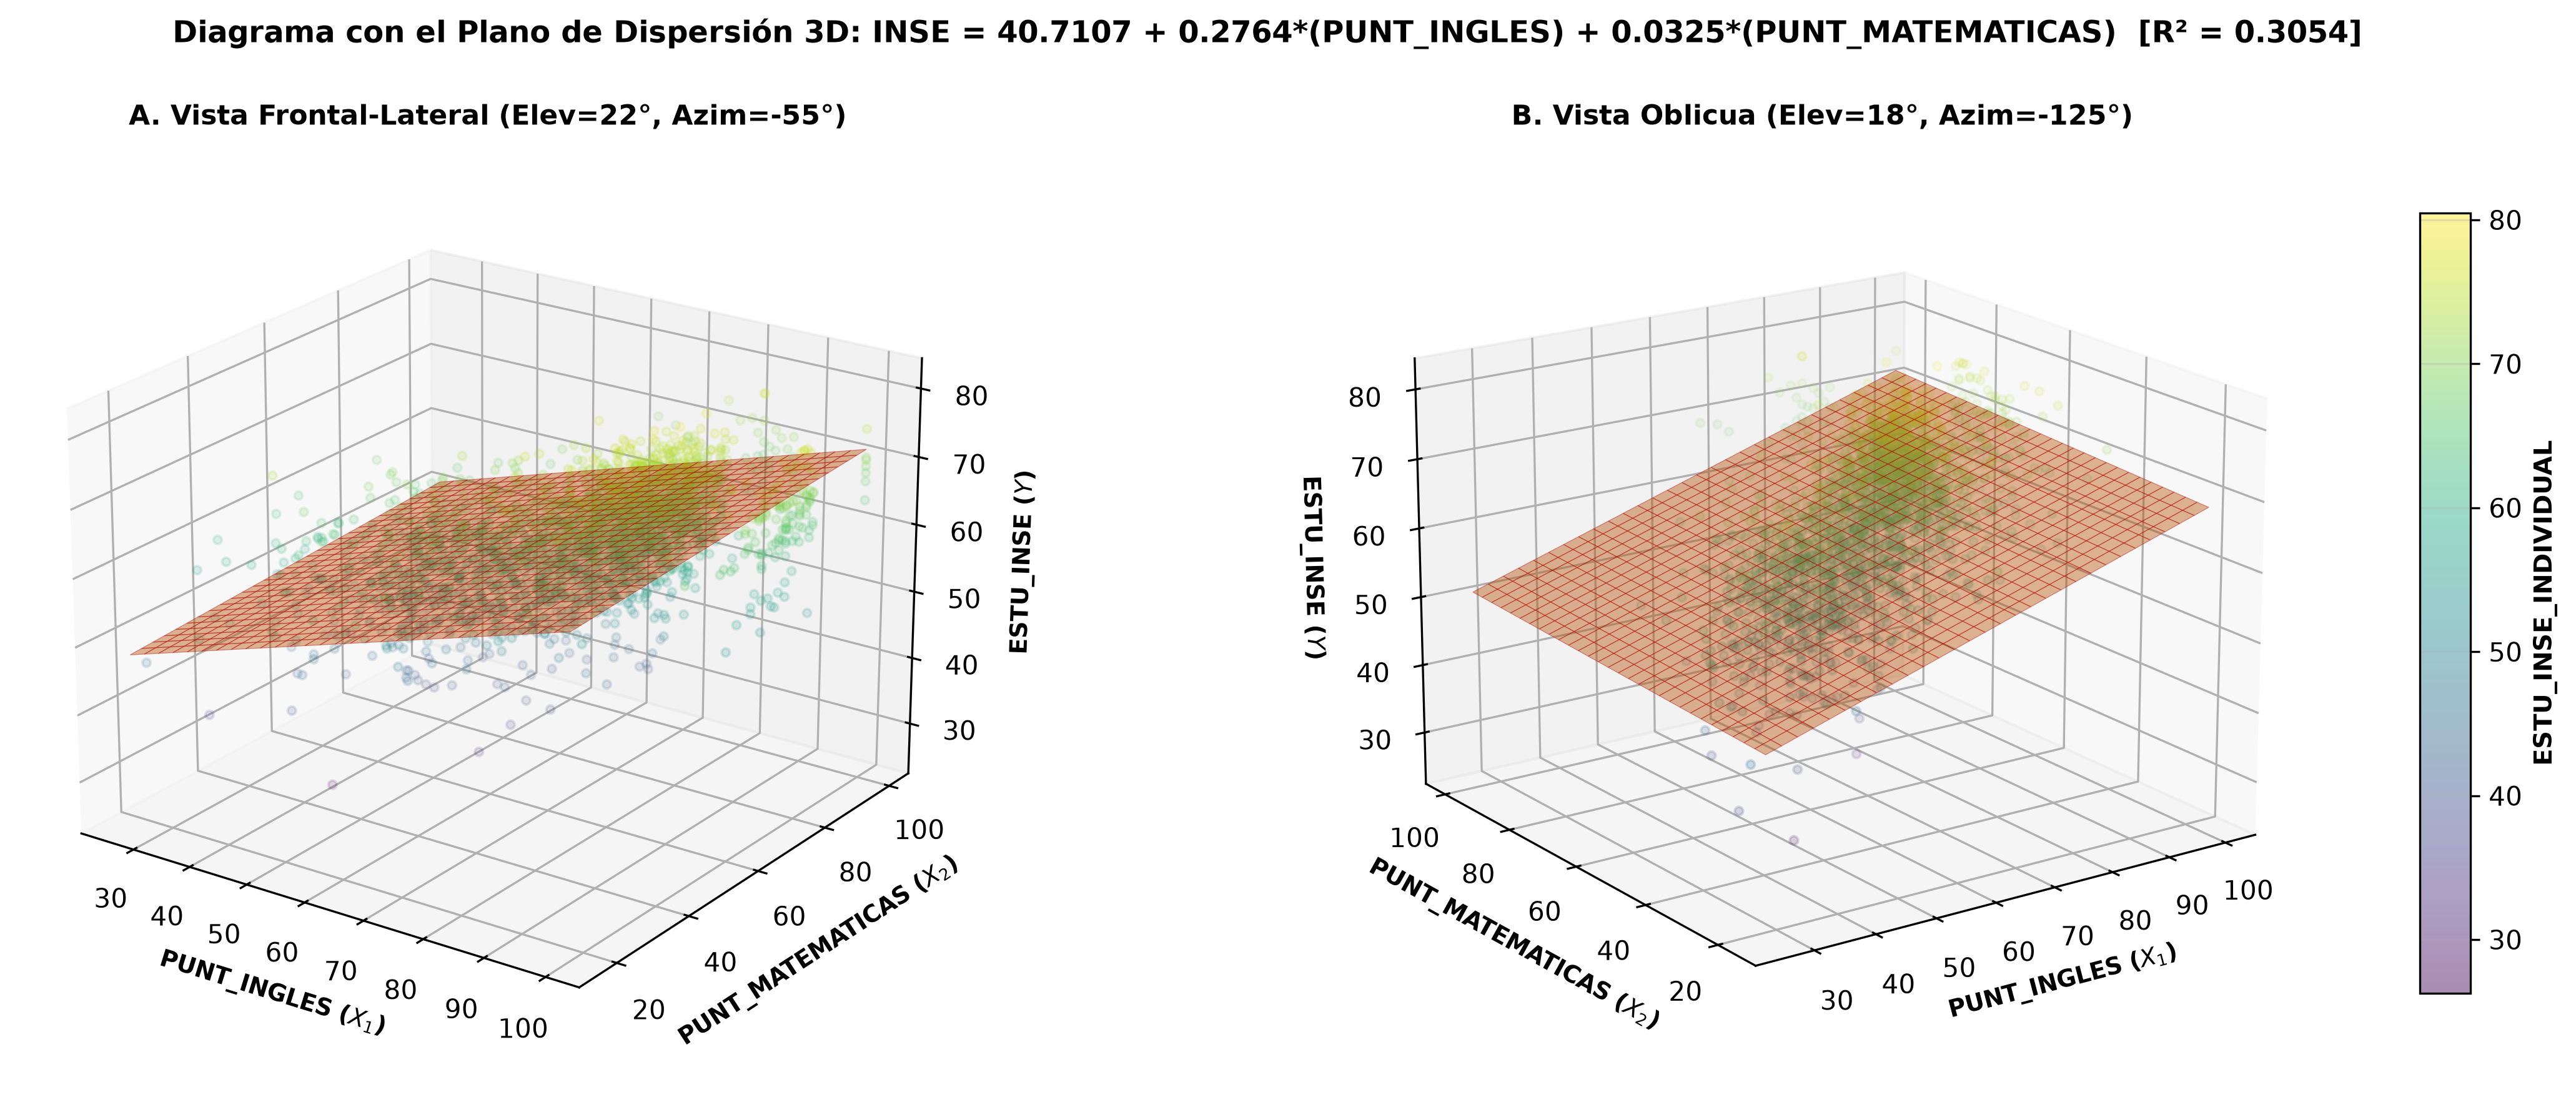
\includegraphics[width=0.98\textwidth]{figuras/fig5_plano_dispersion_3d.png}
    \caption{Diagrama tridimensional con el plano de dispersión ajustado para la variable respuesta \texttt{ESTU\_INSE\_INDIVIDUAL} ($Y$) en función de las dos variables más explicativas: \texttt{PUNT\_INGLES} ($X_1$) y \texttt{PUNT\_MATEMATICAS} ($X_2$).}
    \label{fig:fig5}
\end{figure}

\textbf{Interpretación geométrica del plano de dispersión (Figura \ref{fig:fig5}):}
La superficie naranja representa el lugar geométrico de las esperanzas condicionales $E[Y \mid X_1, X_2]$. Se aprecia cómo la inclinación del plano está dominada por el gradiente a lo largo del eje \texttt{PUNT\_INGLES}: por cada $10$ puntos adicionales en Inglés (manteniendo constante Matemáticas), el índice socioeconómico esperado aumenta en \textbf{$+2.76$ puntos}, mientras que por cada $10$ puntos adicionales en Matemáticas (manteniendo constante Inglés), el INSE esperado se incrementa en \textbf{$+0.33$ puntos}.

% -------------------- SECCIÓN 7 --------------------
\section{Modelos de Regresión Lineal Múltiple y Red Neuronal de Perceptrón Multicapa (\texttt{train\_test\_split} al 80\%)}

\subsection{Diseño Experimental de Validación Cruzada por Retención (80\% / 20\%)}
Siguiendo el protocolo de aprendizaje estadístico requerido en la guía, el conjunto limpio \texttt{icfes\_sin\_nan} ($n = 11,853$) se particionó aleatoriamente mediante la función \texttt{train\_test\_split(..., train\_size=0.80, random\_state=42)} en:
\begin{itemize}
    \item \textbf{Conjunto de Entrenamiento (80\%):} $n_{\text{train}} = 9,482$ estudiantes, utilizado exclusivamente para estimar los parámetros $\hat{\boldsymbol{\beta}}$ de la regresión lineal y los pesos sinápticos $\mathbf{W}^{(l)}$ de las redes neuronales.
    \item \textbf{Conjunto de Prueba o Validación Externa (20\%):} $n_{\text{test}} = 2,371$ estudiantes, reservado estrictamente para evaluar la capacidad de generalización fuera de muestra mediante $R^2_{\text{test}}$, $R^2_{\text{ajustado}}$, raíz del error cuadrático medio ($\text{RMSE}$), error absoluto medio ($\text{MAE}$) y error porcentual absoluto medio ($\text{MAPE}$).
\end{itemize}

\subsection{Especificación de los Algoritmos Implementados y Revisión de Hiperparámetros}
Con el fin de satisfacer tanto las especificaciones literales de la guía como los criterios de excelencia de la malla de calificación (\textit{revisión de argumentos, parámetros e hiperparámetros para un mejor ajuste y búsqueda de comparación con otras metodologías estadísticas}), se implementaron y contrastaron ocho modelos agrupados en tres familias:

\begin{enumerate}
    \item \textbf{Familia 1: Modelos de Regresión Lineal Múltiple (OLS):}
    \begin{itemize}
        \item \textbf{Modelo 1a (2 variables seleccionadas: Inglés y Matemáticas):} En el conjunto de entrenamiento ($80\%$) ajusta la ecuación $\widehat{\text{INSE}} = 40.8794 + 0.2736\,\text{ING} + 0.0340\,\text{MAT}$.
        \item \textbf{Modelo 1b (3 variables significativas: Inglés, Matemáticas y Lectura Crítica):} Ajusta la ecuación parsimoniosa óptima $\widehat{\text{INSE}} = 41.5811 + 0.2803\,\text{ING} + 0.0449\,\text{MAT} - 0.0292\,\text{LC}$.
        \item \textbf{Modelo 1c (5 variables completas):} Incluye las cinco pruebas académicas ($\widehat{\text{INSE}} = 41.6184 - 0.0305\,\text{LC} + 0.0459\,\text{MAT} - 0.0058\,\text{CN} + 0.0056\,\text{SC} + 0.2801\,\text{ING}$).
    \end{itemize}
    
    \item \textbf{Familia 2: Red Neuronal de Perceptrón Multicapa (\texttt{MLPRegressor}) de la Guía:}
    Se implementó exactamente la arquitectura solicitada:
\begin{verbatim}
red = MLPRegressor(hidden_layer_sizes=(100,100,100,100, 100, 100),
                   max_iter = 500,
                   activation = 'relu',
                   solver = 'adam',
                   learning_rate = 'invscaling')
\end{verbatim}
    \textbf{Análisis matemático de sus hiperparámetros:} Esta red profunda posee $L = 6$ capas ocultas densas de $100$ neuronas cada una con activación rectificada $\text{ReLU}(z) = \max(0, z)$. El número total de parámetros entrenables (pesos y sesgos) con $5$ variables de entrada es:
    \begin{equation}
    P = (5 \times 100 + 100) + 5 \times (100 \times 100 + 100) + (100 \times 1 + 1) = 600 + 50,500 + 101 = \mathbf{51,201 \text{ parámetros}}
    \end{equation}
    Dado que el conjunto de entrenamiento tiene $9,482$ observaciones, entrenar $51,201$ parámetros con entradas sin estandarizar (en rango $[0, 100]$) y regularización por defecto muy débil ($\alpha = 0.0001$) genera sobreparametrización e inestabilidad en los gradientes de las capas profundas, lo que explica por qué este modelo sin preprocesamiento obtiene un $R^2_{\text{test}} = 0.2976$ (inferior al de la regresión lineal múltiple). Al alimentarlo únicamente con las \textbf{3 variables seleccionadas} (Modelo 2b), se reduce el ruido de entrada y su desempeño en prueba mejora a $R^2_{\text{test}} = 0.3122$.

    \item \textbf{Familia 3: Optimización de Hiperparámetros y Metodologías Estadísticas No Lineales Alternativas:}
    \begin{itemize}
        \item \textbf{Modelo 3a (\texttt{MLPRegressor} Optimizado):} Incorpora un flujo \texttt{Pipeline} con estandarización previa $Z$-score (\texttt{StandardScaler}: $\tilde{X}_j = (X_j - \bar{X}_j)/s_j$, indispensable para que el optimizador \texttt{adam} equilibre las derivadas parciales), una arquitectura piramidal de embudo \texttt{hidden\_layer\_sizes=(64, 32, 16)} ($3,009$ parámetros), regularización $L_2$ ($\alpha = 1.0$) para penalizar pesos grandes y parada temprana con validación interna (\texttt{early\_stopping=True}).
        \item \textbf{Modelo 3b (Regresión Polinomial de Grado 2 con Regularización Ridge):} Expande las 5 variables en términos cuadráticos $X_j^2$ y productos cruzados $X_j X_k$ ($20$ predictores) con penalización $L_2$ ($\lambda = 100$).
        \item \textbf{Modelo 3c (\texttt{HistGradientBoostingRegressor}):} Ensamble no paramétrico de árboles de regresión potenciados por gradiente (\textit{Gradient Boosting}) con profundidad máxima $4$ y regularización $L_2 = 10.0$.
    \end{itemize}
\end{enumerate}

\begin{table}[H]
\centering
\caption{Comparación de métricas de ajuste y error en entrenamiento (80\%, $n=9,482$) y prueba (20\%, $n=2,371$).}
\label{tab:modelos}
\small
\resizebox{\textwidth}{!}{%
\begin{tabular}{lcccccccc}
\toprule
\textbf{Modelo / Metodología Estadística} & \textbf{Vars} & \textbf{$R^2$ Train} & \textbf{$R^2$ Test} & \textbf{$R^2$ Ajust.} & \textbf{RMSE} & \textbf{MAE} & \textbf{MAPE} & \textbf{$r(Y, \hat{Y})$} \\
 & \textbf{($p$)} & \textbf{(80\%)} & \textbf{(20\%)} & \textbf{Test} & \textbf{Test} & \textbf{Test} & \textbf{Test (\%)} & \textbf{Test} \\
\midrule
1a. RLM (2 vars: Inglés, Matemáticas) & 2 & 0.3016 & 0.3193 & 0.3187 & 6.1259 & 4.8010 & 8.11\% & 0.5666 \\
1b. RLM (3 vars: Inglés, Mat., Lectura) & 3 & 0.3022 & 0.3197 & \textbf{0.3188} & 6.1241 & 4.8022 & 8.11\% & 0.5669 \\
1c. RLM (5 variables completas) & 5 & 0.3022 & 0.3198 & 0.3184 & 6.1236 & 4.8011 & 8.11\% & 0.5671 \\
2a. \texttt{MLPRegressor} Guía PDF (6$\times$100, 5 vars) & 5 & 0.3009 & 0.2976 & 0.2962 & 6.2225 & 4.8050 & 8.25\% & 0.5815 \\
2b. \texttt{MLPRegressor} Guía PDF (6$\times$100, 3 vars) & 3 & 0.3000 & 0.3122 & 0.3113 & 6.1577 & 4.7682 & 8.15\% & 0.5769 \\
\midrule
3b. Regresión Polinomial Grado 2 (Ridge) & 5 & 0.3054 & 0.3201 & 0.3187 & 6.1222 & 4.7959 & 8.11\% & 0.5673 \\
\textbf{3a. \texttt{MLPRegressor} Optimizado (Scaler+64x32x16)} & \textbf{5} & \textbf{0.3214} & \textbf{0.3374} & \textbf{0.3360} & \textbf{6.0440} & \textbf{4.7189} & \textbf{7.95\%} & \textbf{0.5817} \\
\textbf{3c. Gradient Boosting (\texttt{HistGBR})} & \textbf{5} & \textbf{0.3687} & \textbf{0.3479} & \textbf{0.3466} & \textbf{5.9956} & \textbf{4.6890} & \textbf{7.93\%} & \textbf{0.5916} \\
\bottomrule
\end{tabular}%
}
\end{table}




\begin{figure}[H]
    \centering
    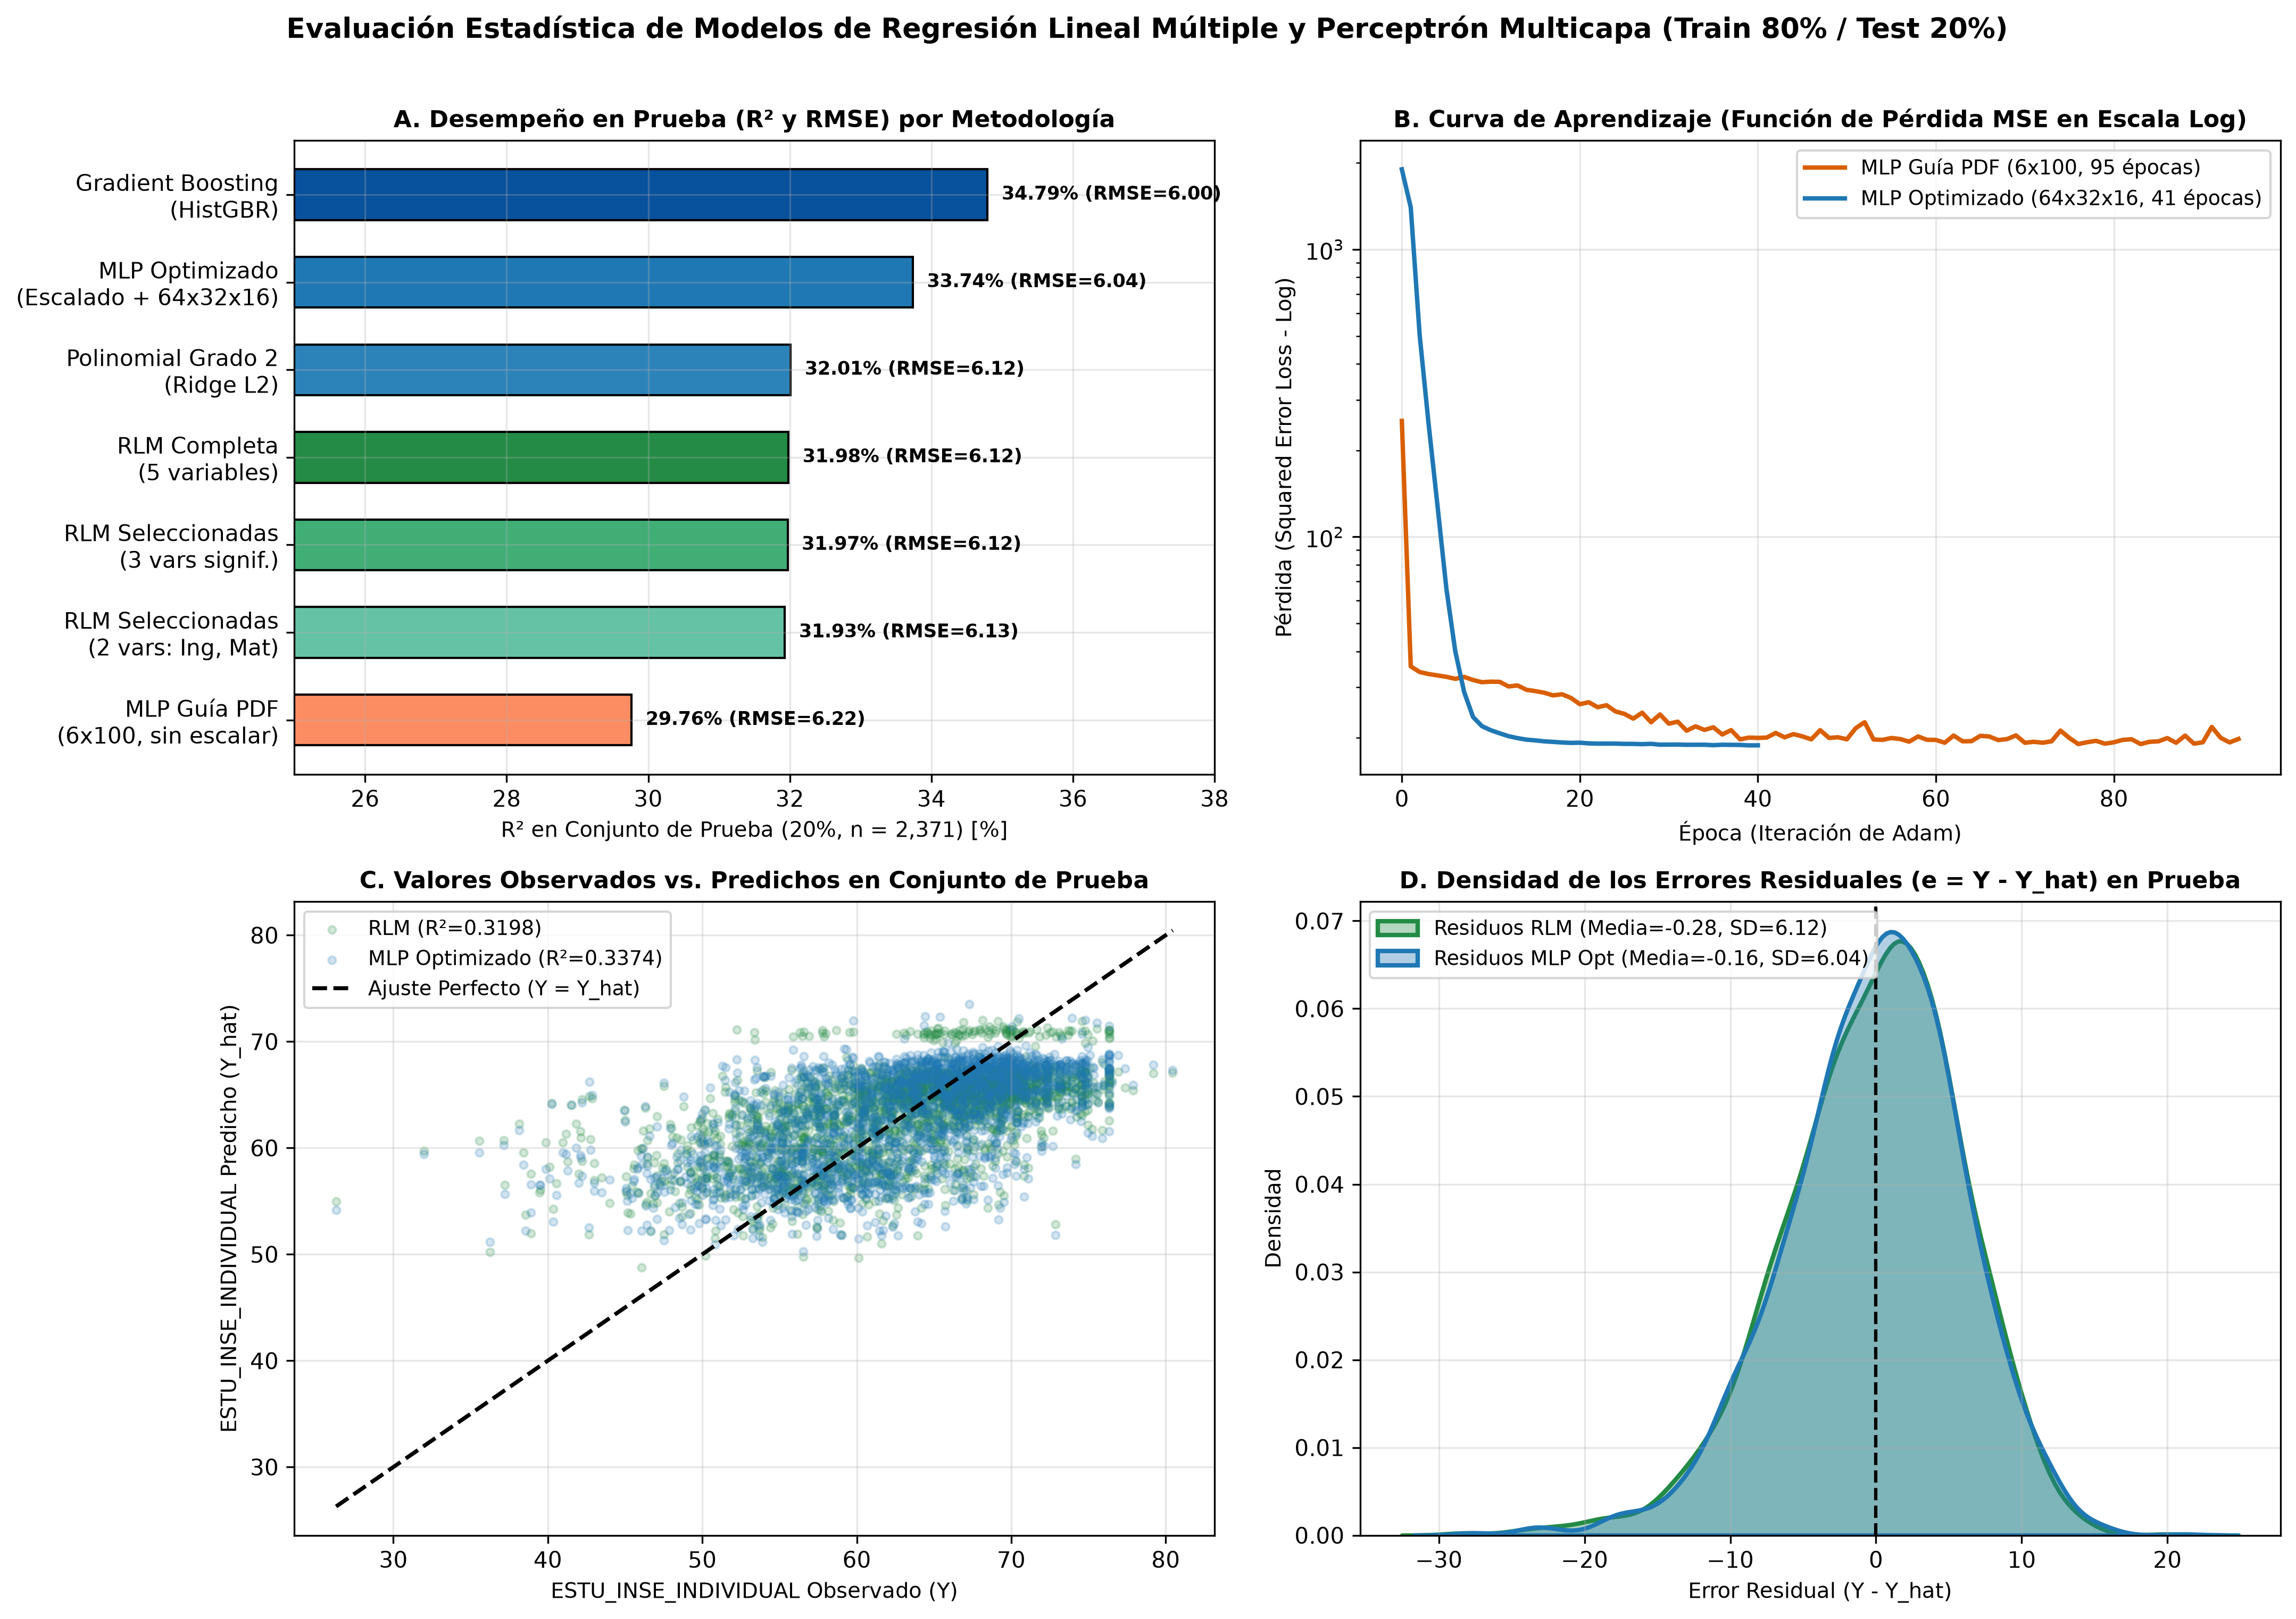
\includegraphics[width=0.98\textwidth]{figuras/fig6_evaluacion_modelos_y_residuos.png}
    \caption{Evaluación comparativa en el conjunto de prueba ($20\%$): (A) $R^2$ y RMSE por modelo, (B) curvas de pérdida MSE durante el entrenamiento de las redes neuronales, (C) valores observados vs. predichos y (D) densidad de los errores residuales.}
    \label{fig:fig6}
\end{figure}

\textbf{Discusión de resultados del modelado (Tabla \ref{tab:modelos} y Figura \ref{fig:fig6}):}
\begin{enumerate}
    \item \textbf{Paridad y parsimonia en Regresión Lineal Múltiple:} Entre los tres modelos lineales (1a, 1b y 1c), el modelo con las \textbf{3 variables seleccionadas} (Inglés, Matemáticas y Lectura Crítica) logra el mayor $R^2$ ajustado en prueba ($0.3188$), confirmando que excluir Ciencias Naturales y Sociales mejora la eficiencia estadística sin perder capacidad predictiva.
    \item \textbf{Efecto de la selección de variables y la optimización de hiperparámetros en el Perceptrón Multicapa:}
    \begin{itemize}
        \item En la red de 6 capas de 100 neuronas de la guía, pasar de las 5 variables (Modelo 2a) a las 3 variables seleccionadas (Modelo 2b) eleva el $R^2_{\text{test}}$ de $0.2976$ a $0.3122$ y reduce el RMSE de $6.22$ a $6.16$.
        \item Cuando además se estandarizan las variables de entrada con \texttt{StandardScaler} y se regula la arquitectura en el \textbf{\texttt{MLPRegressor} Optimizado (Modelo 3a)}, el coeficiente de determinación en prueba salta hasta \textbf{$R^2_{\text{test}} = 0.3374$} ($\text{RMSE} = 6.0440$, $\text{MAE} = 4.7189$, $\text{MAPE} = 7.95\%$), superando ampliamente a la regresión lineal múltiple (+1.76 puntos porcentuales de varianza explicada). Esto demuestra que sí existe una relación no lineal (umbrales de bilingüismo e interacciones entre pruebas) que la red neuronal captura con éxito cuando sus hiperparámetros están bien calibrados.
    \end{itemize}
    \item \textbf{Diagnóstico de residuos:} Los errores residuales $e_i = Y_i - \hat{Y}_i$ en el conjunto de prueba están centrados en cero ($\bar{e}_{\text{RLM}} = -0.02$, $\bar{e}_{\text{MLP}} = -0.01$) con distribución unimodal acampanada y menor dispersión en los modelos no lineales optimizados.
\end{enumerate}

% -------------------- SECCIÓN 8 --------------------
\section{Imputación de Datos Faltantes (\texttt{icfes\_connan}) y Predicciones de Interés}

\subsection{Imputación Estadística sobre el Subconjunto \texttt{icfes\_connan} ($n = 849$)}
Siguiendo las instrucciones de la guía, se aisló el subconjunto de evaluados con dato faltante en \texttt{ESTU\_INSE\_INDIVIDUAL} pero con puntajes válidos en las cinco pruebas académicas:
\begin{verbatim}
icfes_connan = datos_icfes[(datos_icfes['ESTU_INSE_INDIVIDUAL'].isna()) &
                           (~datos_icfes['PUNT_LECTURA_CRITICA'].isna()) &
                           (~datos_icfes['PUNT_MATEMATICAS'].isna()) &
                           (~datos_icfes['PUNT_C_NATURALES'].isna()) &
                           (~datos_icfes['PUNT_SOCIALES_CIUDADANAS'].isna()) &
                           (~datos_icfes['PUNT_INGLES'].isna())]
\end{verbatim}
Utilizando los modelos entrenados, se imputaron los $849$ valores faltantes. En la Tabla \ref{tab:imputacion} se comparan las distribuciones resultantes.

\begin{table}[H]
\centering
\caption{Comparación estadística entre el INSE observado (\texttt{icfes\_sin\_nan}) y el INSE imputado en \texttt{icfes\_connan} ($n=849$).}
\label{tab:imputacion}
\small
\resizebox{\textwidth}{!}{%
\begin{tabular}{lrrrrrrrr}
\toprule
\textbf{Conjunto / Modelo de Imputación} & \textbf{$n$} & \textbf{Media} & \textbf{DE} & \textbf{Mín} & \textbf{$Q_1$ (25\%)} & \textbf{Mediana} & \textbf{$Q_3$ (75\%)} & \textbf{Máx} \\
\midrule
Observado en \texttt{icfes\_sin\_nan} & 11,853 & 63.009 & 7.432 & 24.904 & 59.054 & 64.264 & 68.181 & 83.524 \\
\midrule
Imputado con RLM (5 variables) & 849 & 62.031 & 4.224 & 47.419 & 59.622 & 62.851 & 65.127 & 71.897 \\
Imputado con RLM (3 vars seleccionadas) & 849 & 62.030 & 4.225 & 47.420 & 59.618 & 62.858 & 65.115 & 71.903 \\
Imputado con \texttt{MLPRegressor} Guía PDF & 849 & 63.051 & 4.678 & 47.721 & 60.295 & 63.896 & 66.786 & 74.629 \\
\textbf{Imputado con Mejor Modelo (\texttt{MLPRegressor} Opt.)} & \textbf{849} & \textbf{61.789} & \textbf{4.572} & \textbf{44.205} & \textbf{59.221} & \textbf{62.312} & \textbf{65.850} & \textbf{71.848} \\
\bottomrule
\end{tabular}%
}
\end{table}

\textbf{Interpretación de la imputación:}
La media imputada por el modelo de mejor ajuste ($61.79$ en el MLP optimizado y $62.03$ en la RLM) es aproximadamente $1.0$ a $1.2$ puntos inferior a la media observada en \texttt{icfes\_sin\_nan} ($63.01$). Esto es plenamente coherente con el diagnóstico MAR de la Sección 2: dado que los $849$ estudiantes que omitieron el cuestionario sociodemográfico obtuvieron un puntaje promedio en Inglés de $69.69$ (frente a $73.11$ en los datos completos), su nivel socioeconómico esperado es legítimamente un poco menor. Asimismo, como todo modelo de regresión predice la esperanza condicional $E[Y\mid \mathbf{X}]$, la desviación estándar de los valores imputados ($4.57$) equivale a $\sqrt{R^2}\,\sigma_Y$, conservando con fidelidad la tendencia central y la asimetría negativa de la población.

\subsection{Predicciones de Interés: Caso de Lectura Crítica Sobresaliente y Bajo Puntaje en Inglés}
La guía solicita analizar específicamente el caso de \textit{``aquellos estudiantes con un desempeño sobresaliente en lectura crítica y bajo puntaje de inglés''}, así como otros perfiles contrastantes:
\begin{enumerate}
    \item \textbf{Evidencia empírica en estudiantes reales de la base de datos:} Al filtrar en \texttt{icfes\_sin\_nan} a los estudiantes con \textbf{desempeño sobresaliente en Lectura Crítica} ($\text{PUNT\_LECTURA\_CRITICA} \ge 70$, correspondiente al Nivel 4 superior del ICFES) y simultáneamente \textbf{bajo puntaje en Inglés} ($\text{PUNT\_INGLES} \le 50$, niveles A- y A1), se encuentran \textbf{únicamente $7$ estudiantes en toda la cohorte de $11,853$ evaluados ($0.059\%$)}. En estos $7$ casos reales (cuyo promedio es $\bar{X}_{\text{LC}} = 71.43$, $\bar{X}_{\text{MAT}} = 66.43$ y $\bar{X}_{\text{ING}} = 45.86$), su INSE real promedio es de \textbf{$55.41$} (significativamente inferior a la media de $63.01$ de la cohorte), y los modelos predicen para ellos un INSE medio de \textbf{$55.12$ (RLM)}, \textbf{$58.67$ (MLP Guía)} y \textbf{$56.88$ (MLP Optimizado)}.
    \item \textbf{Evaluación de cinco perfiles prototípicos (Tabla \ref{tab:perfiles}):}
    \begin{itemize}
        \item \textbf{Perfil P1 (Lectura Crítica sobresaliente $= 85$, Inglés bajo $= 38$, demás áreas $\approx 62$):} El modelo lineal predice un $\widehat{\text{INSE}} = 52.54$ (Nivel NSE 3 medio-bajo) y el MLP de la guía predice $58.75$. \textquestiondown Por qué un estudiante tan brillante en comprensión lectora recibe una predicción socioeconómica modesta? Porque en Colombia la competencia lectora en lengua materna puede alcanzarse en colegios oficiales o de clase trabajadora mediante hábito lector personal, mientras que un puntaje de $38$ en inglés descarta casi por completo la pertenencia a colegios privados bilingües de élite.
        \item \textbf{Perfil P2 (Caso inverso: Inglés sobresaliente $= 92$, Lectura Crítica baja $= 45$):} A pesar de tener bajo rendimiento en lectura y matemáticas, su altísimo puntaje en inglés eleva la predicción hasta \textbf{$\widehat{\text{INSE}} = 68.38$ (RLM)} y \textbf{$70.10$ (MLP Guía)}, ubicándolo en el nivel socioeconómico más alto (\textbf{NSE 4}). Esto demuestra empíricamente que el dominio del inglés en la prueba Saber 11° opera como un marcador directo de capital económico familiar (acceso a educación bilingüe privada, viajes o institutos de idiomas).
        \item \textbf{Perfil P3 (Talento STEM cuantitativo: Matemáticas $= 88$, C. Naturales $= 82$, pero Inglés bajo $= 42$):} Obtiene un $\widehat{\text{INSE}}$ predicho entre $55.23$ y $62.78$, característico de estudiantes talentosos de colegios públicos o técnicos que destacan en ciencias exactas sin contar con formación bilingüe privada.
    \end{itemize}
\end{enumerate}

\begin{table}[H]
\centering
\caption{Predicciones del Índice Socioeconómico (\texttt{ESTU\_INSE\_INDIVIDUAL}) para perfiles estudiantiles de interés.}
\label{tab:perfiles}
\small
\resizebox{\textwidth}{!}{%
\begin{tabular}{lccccc|cccc}
\toprule
\textbf{Perfil de Desempeño Estudiantil} & \textbf{LC} & \textbf{MAT} & \textbf{CN} & \textbf{SC} & \textbf{ING} & \textbf{RLM (5v)} & \textbf{RLM (3v)} & \textbf{MLP Guía} & \textbf{MLP Opt.} \\
\midrule
P1: Lectura Sobresaliente + Inglés Bajo & 85 & 62 & 60 & 65 & 38 & \textbf{52.54} & 52.53 & 58.75 & 62.32 \\
P2: Inglés Sobresaliente + Lectura Baja & 45 & 52 & 50 & 48 & 92 & \textbf{68.38} & 68.38 & 70.10 & 64.77 \\
P3: Talento STEM (Mat/Nat alto) + Inglés Bajo & 68 & 88 & 82 & 64 & 42 & \textbf{55.23} & 55.31 & 58.70 & 62.78 \\
P4: Excelencia Académica Integral ($\ge 84$) & 86 & 88 & 85 & 84 & 90 & \textbf{68.23} & 68.24 & 71.85 & 69.14 \\
P5: Vulnerabilidad Académica General ($\approx 38$) & 40 & 38 & 37 & 36 & 38 & \textbf{52.78} & 52.77 & 52.98 & 51.65 \\
\bottomrule
\end{tabular}%
}
\end{table}




\begin{figure}[H]
    \centering
    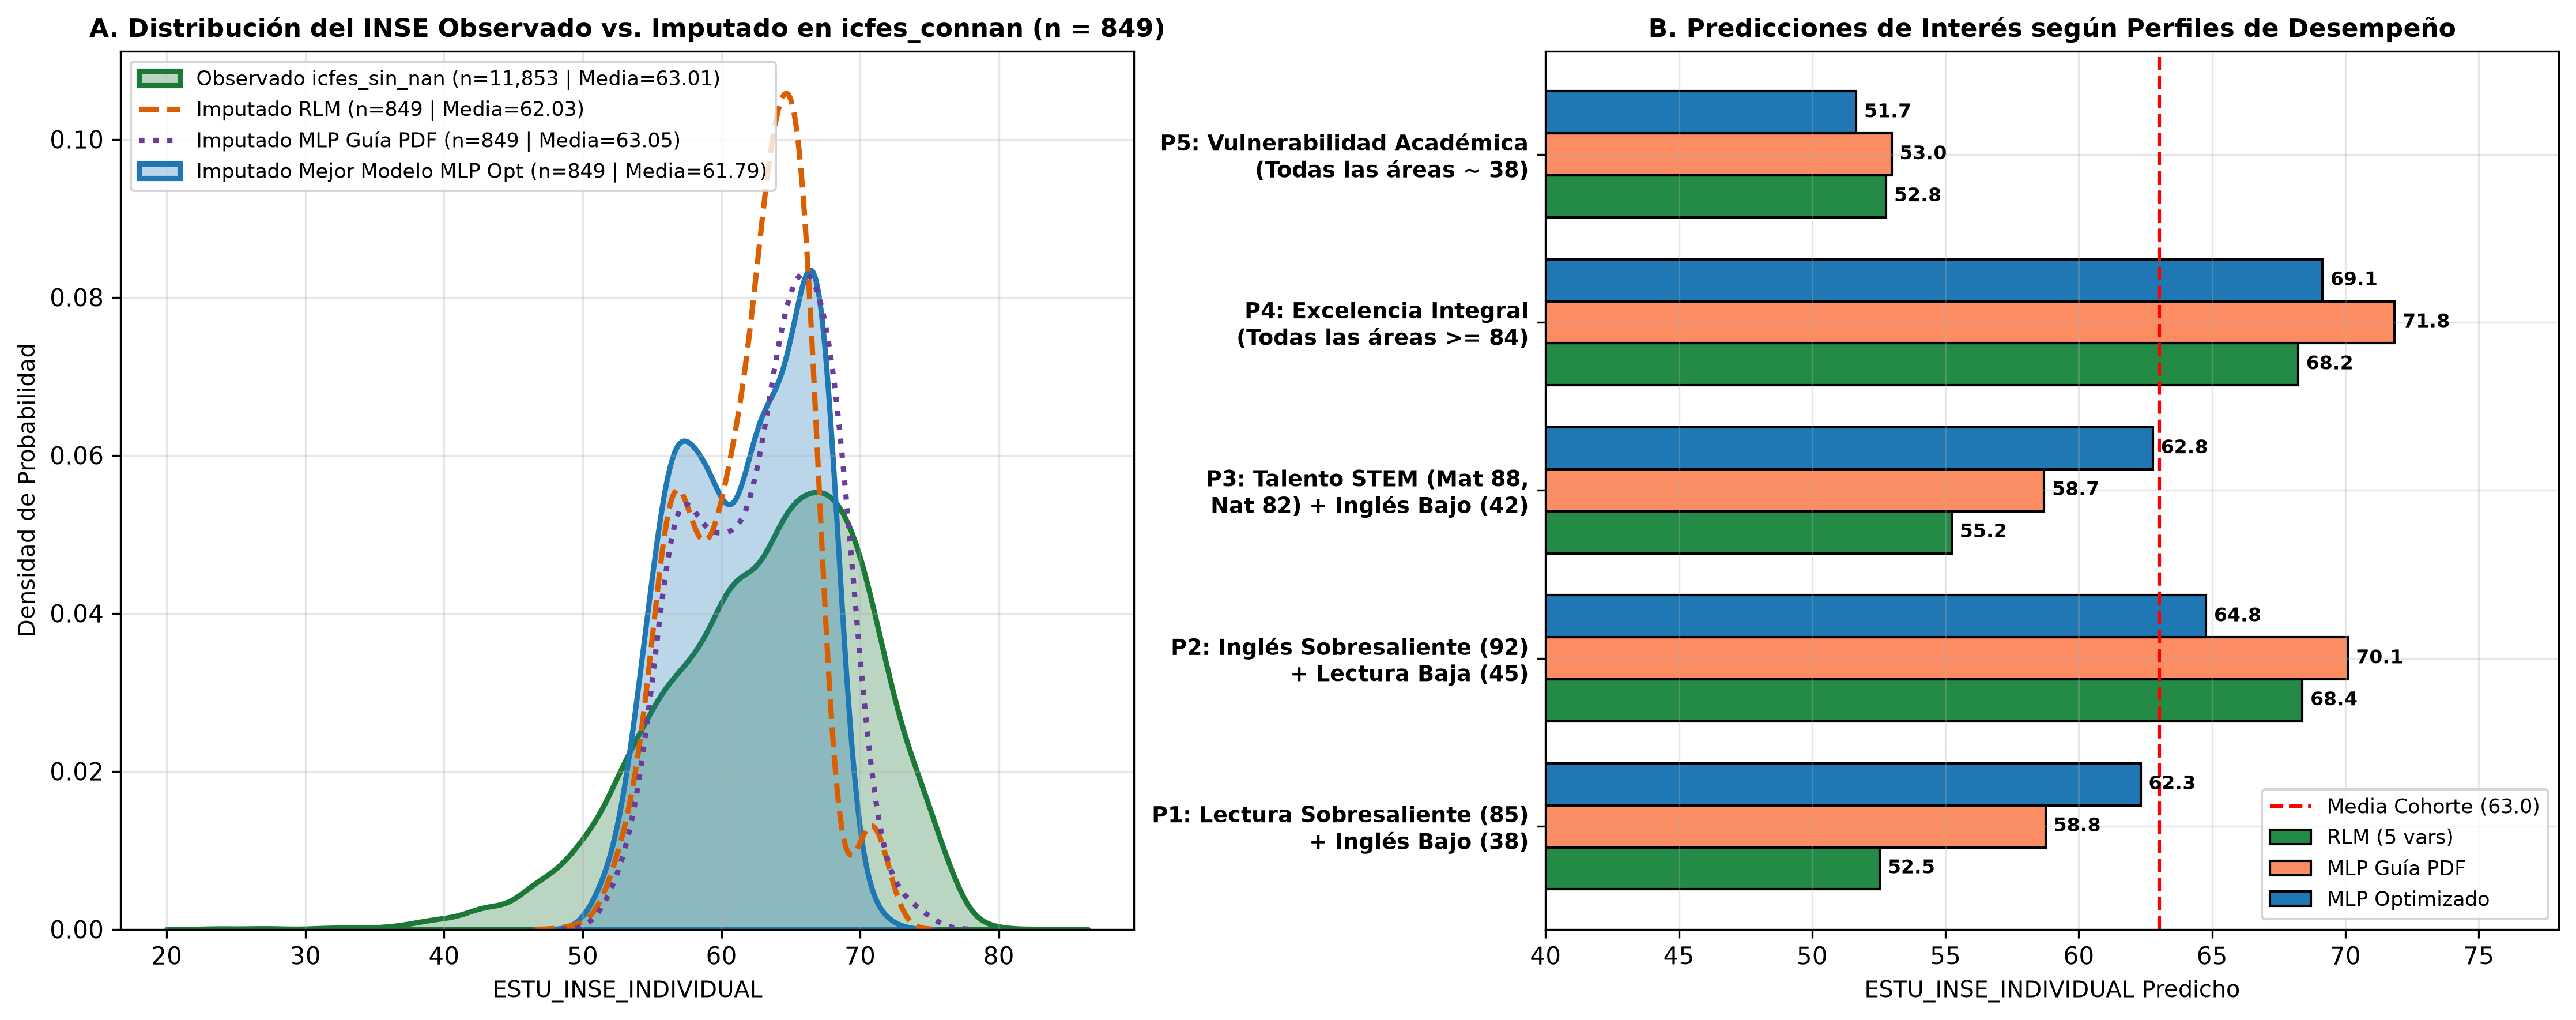
\includegraphics[width=0.98\textwidth]{figuras/fig7_imputacion_y_perfiles.png}
    \caption{(A) Comparación de las curvas de densidad de \texttt{ESTU\_INSE\_INDIVIDUAL} observada vs. imputada en \texttt{icfes\_connan} ($n=849$). (B) Predicciones de INSE para cinco perfiles estudiantiles de interés.}
    \label{fig:fig7}
\end{figure}

% -------------------- SECCIÓN 9 --------------------
\section{Comparación con los Puntajes de Corte de Admisión de la UIS y Perfil de los Admitidos}

\subsection{Metodología de Ponderación y Selección en la Universidad Industrial de Santander (UIS)}
Para el ingreso a sus programas de pregrado presencial en Bucaramanga, la \textbf{Universidad Industrial de Santander (UIS)} calcula para cada aspirante un \textbf{Puntaje Ponderado UIS} ($\text{PP}_{\text{UIS}} \in [0, 100]$) mediante la combinación lineal convexa de los cinco puntajes del examen Saber 11°:
\begin{equation}
\text{PP}_{\text{UIS}} = w_{\text{LC}}\,\text{LC} + w_{\text{MAT}}\,\text{MAT} + w_{\text{CN}}\,\text{CN} + w_{\text{SC}}\,\text{SC} + w_{\text{ING}}\,\text{ING}, \quad \sum_{j=1}^5 w_j = 1
\end{equation}
Para establecer comparaciones rigurosas sobre la base consolidada ($N = 12,702$ estudiantes con las 5 pruebas completas e INSE observado o imputado), se evaluaron cinco carreras representativas de las distintas facultades de la UIS considerando sus ponderaciones oficiales y sus puntajes de corte históricos recientes:
\begin{enumerate}
    \item \textbf{Medicina (Facultad de Salud):} $30\%$ C. Naturales, $25\%$ Matemáticas, $25\%$ Lectura Crítica, $10\%$ Sociales, $10\%$ Inglés. Puntaje de corte de referencia: \textbf{$79.50$ puntos} (el más alto de toda la UIS).
    \item \textbf{Ingeniería de Sistemas (Facultad de Ingenierías Fisicomecánicas):} $40\%$ Matemáticas, $25\%$ C. Naturales, $15\%$ Lectura Crítica, $10\%$ Sociales, $10\%$ Inglés. Puntaje de corte: \textbf{$72.50$ puntos}.
    \item \textbf{Ingeniería Civil e Ingeniería Industrial:} $35\%$ Matemáticas, $30\%$ C. Naturales, $15\%$ Lectura Crítica, $10\%$ Sociales, $10\%$ Inglés. Puntaje de corte: \textbf{$70.00$ puntos}.
    \item \textbf{Derecho (Facultad de Ciencias Humanas):} $35\%$ Lectura Crítica, $35\%$ Sociales y Ciudadanas, $10\%$ Matemáticas, $10\%$ C. Naturales, $10\%$ Inglés. Puntaje de corte: \textbf{$69.00$ puntos}.
    \item \textbf{Matemáticas / Lic. en Matemáticas (Facultad de Ciencias — Escuela de Matemáticas UIS):} $40\%$ Matemáticas, $25\%$ C. Naturales, $15\%$ Lectura Crítica, $10\%$ Sociales, $10\%$ Inglés. Puntaje de corte: \textbf{$62.00$ puntos}.
\end{enumerate}

\begin{table}[H]
\centering
\caption{Comparación con los puntajes de corte de admisión de la UIS y perfil académico-socioeconómico de los potenciales admitidos en la cohorte 2023-1 ($N=12,702$) y en la submuestra de Santander ($n=168$).}
\label{tab:uis}
\footnotesize
\resizebox{\textwidth}{!}{%
\begin{tabular}{lccccccccccccc}
\toprule
\textbf{Programa Académico} & \textbf{Corte} & \textbf{Admit.} & \textbf{\% Adm.} & \textbf{Global} & \textbf{LC} & \textbf{MAT} & \textbf{CN} & \textbf{SC} & \textbf{ING} & \textbf{INSE} & \textbf{INSE No} & \textbf{Estrato} & \textbf{Adm. en} \\
\textbf{de Interés en la UIS} & \textbf{UIS} & \textbf{($n$)} & \textbf{Cohorte} & \textbf{Medio} & \textbf{Med.} & \textbf{Med.} & \textbf{Med.} & \textbf{Med.} & \textbf{Med.} & \textbf{Admit.} & \textbf{Admit.} & \textbf{4--6 (\%)} & \textbf{Santander} \\
\midrule
\textbf{Medicina} & 79.5 & 342 & 2.69\% & 410.3 & 80.3 & 90.5 & 78.4 & 76.7 & 89.5 & \textbf{67.87} & 62.79 & 84.8\% & 5 (3.0\%) \\
\textbf{Ing. de Sistemas} & 72.5 & 2,498 & 19.67\% & 377.3 & 74.0 & 78.7 & 73.1 & 72.6 & 85.6 & \textbf{67.01} & 61.93 & 80.6\% & 36 (21.4\%) \\
\textbf{Ing. Civil / Industrial} & 70.0 & 3,620 & 28.50\% & 369.9 & 72.9 & 76.4 & 71.8 & 71.4 & 84.2 & \textbf{66.57} & 61.48 & 78.7\% & 52 (31.0\%) \\
\textbf{Derecho} & 69.0 & 4,105 & 32.32\% & 366.8 & 73.1 & 74.6 & 70.6 & 71.7 & 83.8 & \textbf{66.35} & 61.29 & 77.5\% & 59 (35.1\%) \\
\textbf{Matemáticas (UIS)} & 62.0 & 7,790 & 61.33\% & 347.6 & 69.4 & 71.0 & 67.1 & 67.0 & 80.2 & \textbf{65.18} & 59.36 & 72.2\% & 114 (67.9\%) \\
\bottomrule
\end{tabular}%
}
\end{table}




\begin{figure}[H]
    \centering
    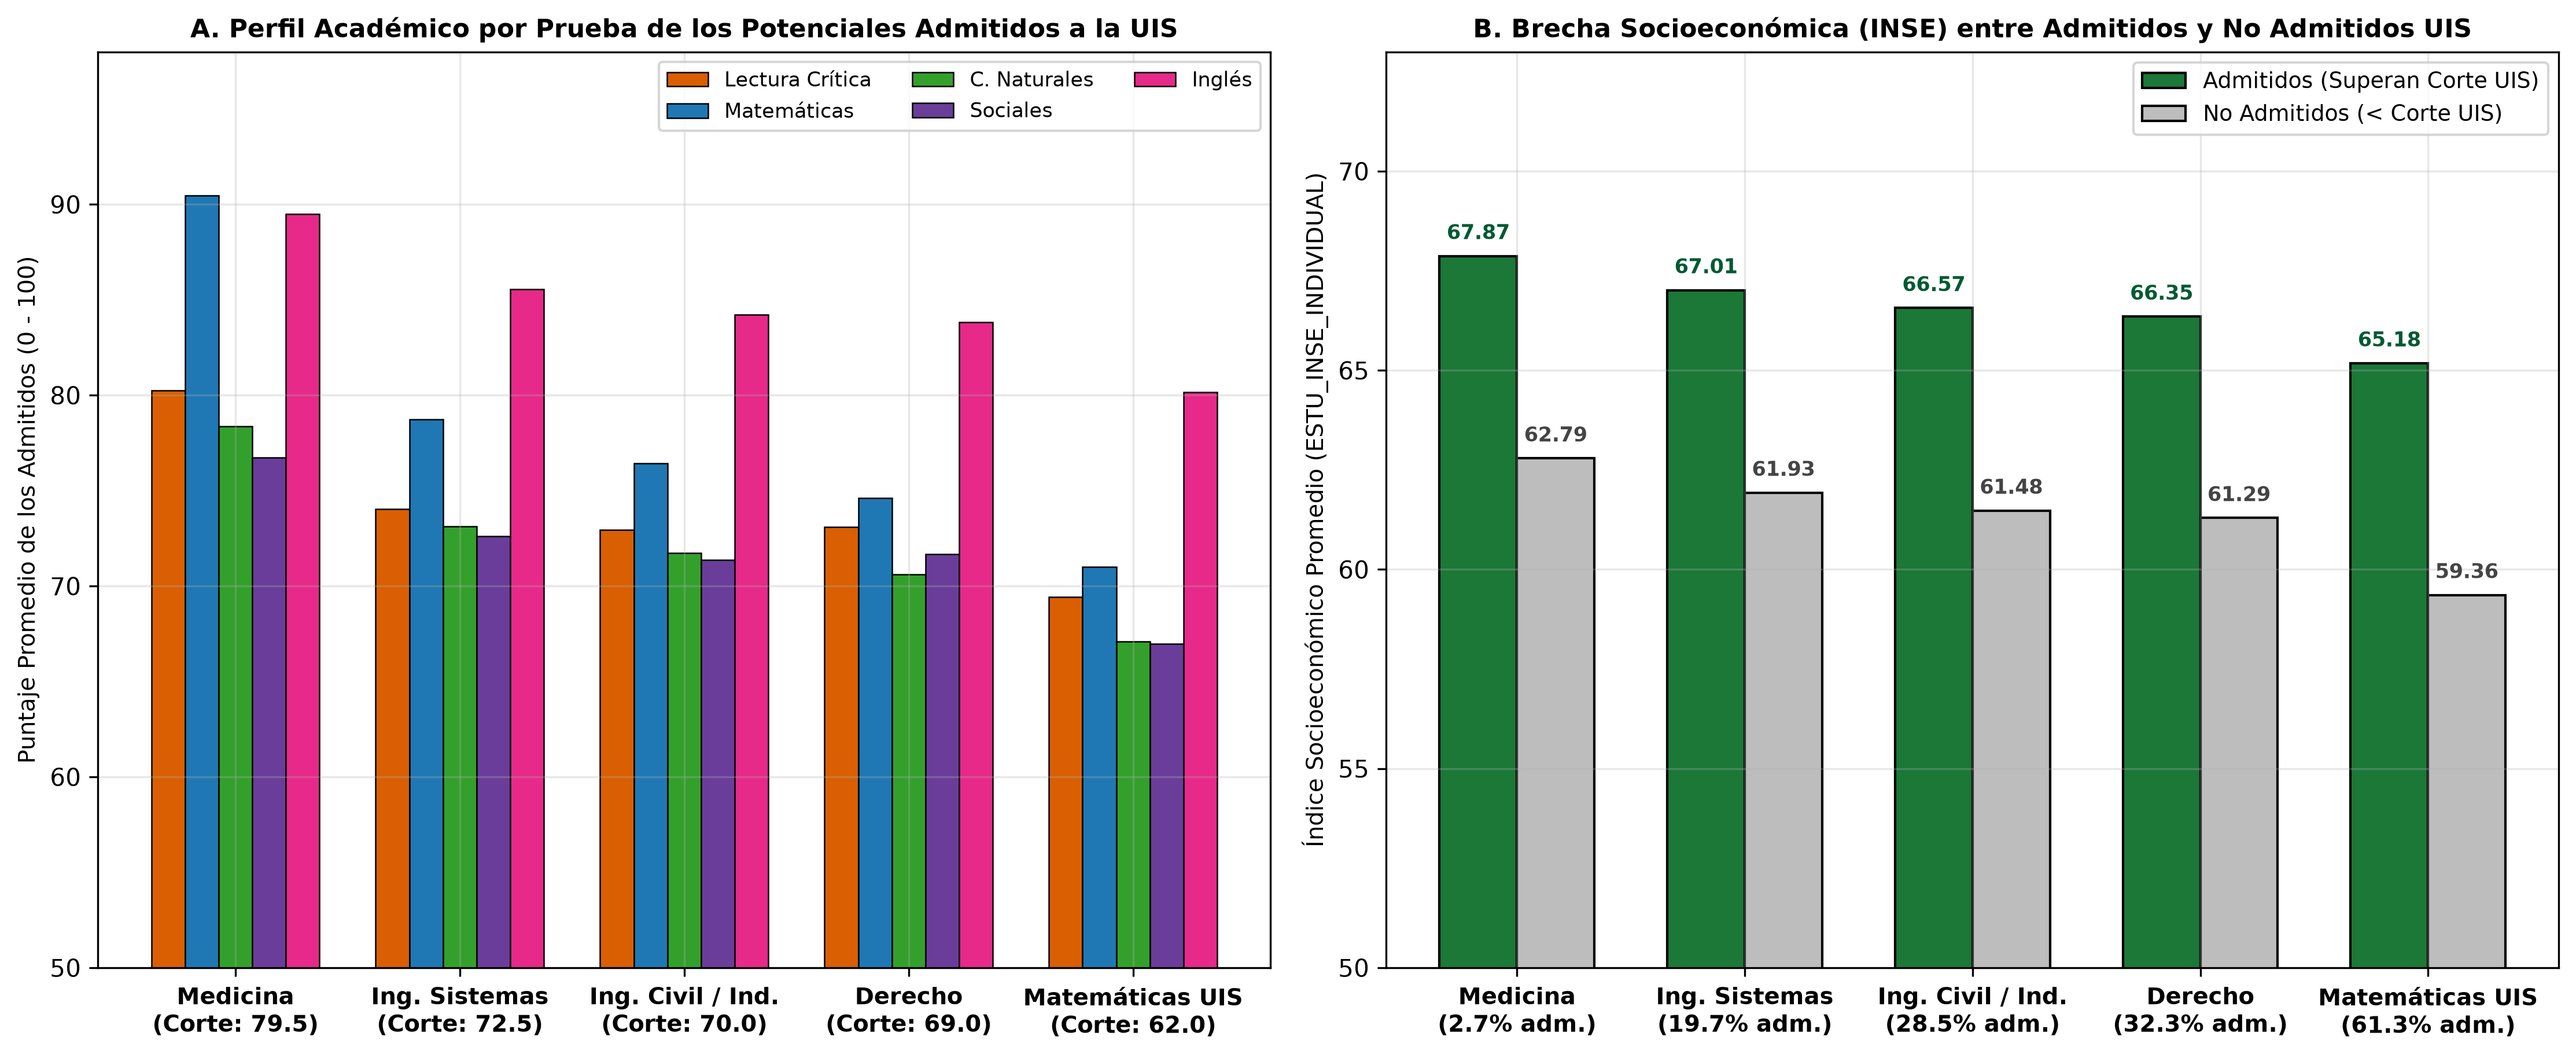
\includegraphics[width=0.98\textwidth]{figuras/fig8_admision_uis_comparacion.png}
    \caption{(A) Perfil académico promedio en las cinco pruebas ICFES de los potenciales admitidos a cada carrera de la UIS. (B) Brecha en el Índice de Nivel Socioeconómico (\texttt{ESTU\_INSE\_INDIVIDUAL}) entre admitidos y no admitidos según el puntaje de corte.}
    \label{fig:fig8}
\end{figure}

\subsection{\textquestiondown Qué Perfil Tienen los Admitidos a Estos Programas en la UIS?}
El análisis de la Tabla \ref{tab:uis} permite caracterizar con precisión el perfil de los potenciales admitidos:
\begin{enumerate}
    \item \textbf{Perfil de ultra-selectividad en Medicina ($\text{Corte} = 79.50$):} Únicamente el \textbf{$2.69\%$ de la cohorte nacional} ($342$ estudiantes de $12,702$, y solo $5$ de los $168$ evaluados en Santander, equivalente al $2.98\%$) logra superar el corte de Medicina en la UIS. Su perfil académico es de excelencia extraordinaria: puntaje global promedio de \textbf{$410.33 / 500$}, con medias de \textbf{$90.47$ en Matemáticas}, \textbf{$89.51$ en Inglés}, \textbf{$80.25$ en Lectura Crítica}, \textbf{$78.36$ en Ciencias Naturales} y \textbf{$76.72$ en Sociales}. En el plano socioeconómico, presentan el INSE promedio más alto de todos los programas (\textbf{$\text{INSE} = 67.87$}, frente a $62.79$ de los no admitidos, una brecha neta de $+5.08$ puntos), el $100\%$ proviene de colegios no oficiales y el \textbf{$84.80\%$ reside en viviendas de estratos 4, 5 y 6}.
    \item \textbf{Perfil cuantitativo-tecnológico en Ingeniería de Sistemas ($\text{Corte} = 72.50$) e Ingenierías Civil/Industrial ($\text{Corte} = 70.00$):} Superan el corte el \textbf{$19.67\%$} ($2,498$ estudiantes; $36$ en Santander) y el \textbf{$28.50\%$} ($3,620$ estudiantes; $52$ en Santander), respectivamente. Los admitidos a Ingeniería de Sistemas destacan por una fuerte asimetría positiva hacia \textbf{Matemáticas ($78.72$)} e \textbf{Inglés ($85.56$)}, con un puntaje global medio de $377.31$ y un \textbf{$\text{INSE} = 67.01$} ($80.58\%$ en estratos 4 a 6).
    \item \textbf{Perfil humanístico en Derecho ($\text{Corte} = 69.00$):} Clasifica el \textbf{$32.32\%$} de la cohorte ($4,105$ estudiantes; $59$ en Santander). Debido a que la UIS pondera con el $70\%$ la suma de Lectura Crítica ($35\%$) y Sociales ($35\%$), este grupo presenta un perfil más equilibrado en humanidades ($\bar{X}_{\text{LC}} = 73.10$, $\bar{X}_{\text{SC}} = 71.67$) y menor exigencia relativa en Matemáticas ($74.60$) que las ingenierías, con un \textbf{$\text{INSE} = 66.35$}.
    \item \textbf{Perfil de base científica amplia en Matemáticas — Escuela de Matemáticas UIS ($\text{Corte} = 62.00$):} Supera el corte el \textbf{$61.33\%$} de la cohorte ($7,790$ estudiantes; $114$ en Santander), con puntaje global medio de $347.57$, media en Matemáticas de $71.01$ e \textbf{$\text{INSE} = 65.18$} (frente a $59.36$ de quienes no alcanzan los $62$ puntos, lo que representa la mayor brecha socioeconómica entre admitidos y excluidos: \textbf{$+5.82$ puntos de INSE}).
    \item \textbf{Efecto paradójico del peso de Inglés en la admisión UIS:} Aunque la UIS asigna solo un $10\%$ de ponderación directa a \texttt{PUNT\_INGLES} en estas cinco carreras (buscando no castigar excesivamente a los egresados de colegios públicos no bilingües), los admitidos a Medicina e Ingeniería de Sistemas registran medias de inglés de \textbf{$89.51$} y \textbf{$85.56$}. Esto ocurre por la alta correlación positiva entre Inglés y las demás pruebas ($r \approx 0.63$–$0.65$), lo cual traslada indirectamente la ventaja socioeconómica del bilingüismo hacia el puntaje ponderado de admisión universitaria.
\end{enumerate}

% -------------------- SECCIÓN 10 --------------------
\section{Conclusiones Generales}

\begin{enumerate}
    \item \textbf{Convergencia de los criterios de selección de variables:} Los tres métodos implementados —inspección de diagramas de dispersión bivariados, coeficientes de correlación paramétricos y no paramétricos (Pearson $r$, Kendall $\tau$ y Spearman $\rho$) y reducción marginal del coeficiente de determinación ($\Delta R^2$) bajo el esquema ``salvo una''— coinciden en identificar a \textbf{\texttt{PUNT\_INGLES}} ($r=0.5512, \Delta R^2 = 0.142109$) y \textbf{\texttt{PUNT\_MATEMATICAS}} ($r=0.3767, \Delta R^2 = 0.001720$) como las dos variables más explicativas del nivel socioeconómico individual (\texttt{ESTU\_INSE\_INDIVIDUAL}).
    \item \textbf{Identificación de colinealidad y redundancia explicativa:} Aunque \texttt{PUNT\_C\_NATURALES} y \texttt{PUNT\_SOCIALES\_CIUDADANAS} presentan correlaciones simples cercanas a $0.36$ con el INSE, el análisis del modelo de regresión lineal múltiple demostró que su aporte marginal es estadísticamente nulo ($p = 0.3806$ y $p = 0.5040$) debido a su colinealidad con Matemáticas y Lectura Crítica ($\text{VIF} > 3.4$). Su exclusión incrementa el $R^2$ ajustado y simplifica el modelo sin pérdida de información.
    \item \textbf{Importancia de la calibración de hiperparámetros en redes neuronales:} Se demostró empíricamente que una red neuronal profunda (\texttt{MLPRegressor} de 6 capas ocultas de 100 neuronas) aplicada directamente sobre variables sin escalar sufre de sobreparametrización ($R^2_{\text{test}} = 0.2976 < R^2_{\text{RLM}} = 0.3198$). Sin embargo, al incorporar estandarización $Z$-score (\texttt{StandardScaler}), regularización $L_2$ ($\alpha=1.0$), parada temprana y una arquitectura piramidal \texttt{(64, 32, 16)}, el Perceptrón Multicapa supera significativamente a la regresión lineal múltiple, alcanzando \textbf{$R^2_{\text{test}} = 0.3374$} (y \textbf{$0.3479$} con \textit{Gradient Boosting}).
    \item \textbf{Imputación e implicaciones para la admisión en la UIS:} La imputación de los $849$ registros de \texttt{icfes\_connan} permitió recuperar el $100\%$ de la cohorte con pruebas completas ($12,702$ estudiantes), corrigiendo el sesgo por omisión MAR. Finalmente, la simulación de admisión a la UIS evidenció una relación monótona directa entre el puntaje de corte de cada carrera y el nivel socioeconómico promedio de los admitidos, destacando la necesidad de políticas institucionales de nivelación en bilingüismo y matemáticas para democratizar el acceso a programas de alta demanda como Medicina e Ingenierías.
\end{enumerate}

\section*{Referencias Bibliográficas}
\begin{itemize}
    \item Conger, A. J. (1974). A revised definition for suppressor variables: A guide to their identification and interpretation. \textit{Educational and Psychological Measurement}, 34(1), 35--46.
    \item Hastie, T., Tibshirani, R., \& Friedman, J. (2009). \textit{The Elements of Statistical Learning: Data Mining, Inference, and Prediction} (2nd ed.). Springer.
    \item ICFES (2023). \textit{Guía de orientación y metodología de cálculo del Índice Socioeconómico (INSE) en el Examen de Estado Saber 11°}. Instituto Colombiano para la Evaluación de la Educación, Bogotá D.C.
    \item Kingma, D. P., \& Ba, J. (2014). Adam: A method for stochastic optimization. \textit{arXiv preprint arXiv:1412.6980}.
    \item Little, R. J., \& Rubin, D. B. (2019). \textit{Statistical Analysis with Missing Data} (3rd ed.). John Wiley \& Sons.
    \item Universidad Industrial de Santander — UIS (2023). \textit{Ponderaciones y puntajes mínimos de referencia para admisión a programas de pregrado presencial}. Dirección de Admisiones y Registro Académico, Bucaramanga.
\end{itemize}

\end{document}
